\documentclass[a4paper,10pt, oneside]{article}
\usepackage[utf8]{inputenc}
\usepackage[spanish]{babel}
\usepackage[style=ieee,backend=bibtex]{biblatex}
\usepackage{graphicx}
\usepackage{amsmath}
\usepackage{pgfplots}
\usepackage{lineno}
\usepackage{amsmath}
\usepackage[top=1in, bottom=1.25in, left=1.25in, right=1.25in]{geometry}
\usepackage{caption}
\usepackage{bytefield}
\usepackage{amsmath}
\usepackage{csquotes}
\usepackage{svg}
\usepackage{lscape}
\usepackage{draftwatermark}
\usepackage{svg}
\usepackage{multicol}
\usepackage{pgfplots, pgfplotstable}
\usepackage{amsmath,amsthm}
\usepackage{hyperref}
\newtheorem{theorem}{Teorema}[section]
\newtheorem{lemma}[theorem]{Lema}


\SetWatermarkScale{5}
\SetWatermarkColor[gray]{0.95}
\usepackage{bytefield}
\graphicspath{ {graph/} }



\usepackage[linesnumbered,ruled]{algorithm2e}


\bibliography{informe_final}
	
\begin{document}
	
\begin{titlepage}
	\centering
	
\includegraphics[width=0.25\textwidth]{../Universidad_del_Litoral}\par\vspace{1cm}
	{\scshape\LARGE Universidad Nacional del Litoral \par}
	\vspace{1cm}
	{\scshape\Large Proyecto Final de Carrera\par}
	\vspace{1.5cm}
	{\huge\bfseries Diseño de un sistema de detección de anomalías en redes de computadoras.\par}
	\vspace{4cm}
	{\huge\bfseries Informe Final\par}
	\vfill
	
	{\Large \itshape Pineda Leandro\par}
	
	
	% Bottom of the page
	\large Córdoba\par
	{\large \today\par}	
\end{titlepage}

\modulolinenumbers[5]
\linenumbers


\clearpage\mbox{}\clearpage
\tableofcontents

\newpage

\section{Introducción}
En la actualidad, \textit{BigData} es uno de los tantos conceptos de moda en el mundo informático. Este se usa para hacer referencia a grandes colecciones de datos que pueden crecer a volúmenes enormes y a un ritmo tan alto que resulta difícil o imposible manejarlos con las herramientas tradicionales, como las bases de datos relaciones convencionales. El desafío que presenta el \textit{BigData} no solo está limitado a los aspectos técnicos de almacenar cantidades masivas de datos, sino en cómo obtener de estos información relevante que permitan asistir a la toma de decisiones.
Este concepto comenzó a tomar fuerza a principios del año 2000 cuando Doug Laney, vicepresidente y analista distinguido de Gartner\footnote{Gartner Inc. es una empresa consultora y de investigación de las tecnologías de la información con sede en Stamford, Connecticut, Estados Unidos}, caracterizó al \textit{BigData} mediante tres V:
\begin{itemize}
	\item Volumen: Las organizaciones recolectan cantidad masivas de datos de diversas fuentes (transacciones, social-media, sensores, etc). En el pasado, almacenar tal volumen de datos hubiese sido un problema, pero nuevas tecnologías como \textit{Hadoop} surgieron para hacer frente al desafío.
	\item Velocidad: Los datos se generan cada vez a mayor velocidad, y deben ser manejados en un tiempo aceptable. Etiquetas RFID, sensores y dispositivos IoT, entre otros, hacen que sea necesario procesar estos flujos de datos rápidamente.
	\item Variedad: Los datos vienen en todo tipo de formatos (estructurados, semi-estructurados o sin estructura).
\end{itemize}

Dependiendo de la necesidad de negocios particular de cada empresa o entidad y la naturaleza de los datos, una de las tres V descritas puede ser más importante que las otras. Si se quiere hacer un pronóstico para cierta actividad, por ejemplo, será necesario contar con grandes volúmenes de datos del pasado. Por el contrario, si es necesario entender cómo varía cierto patrón en los datos en una ventana de tiempo cercana a la presente, será necesario procesarlos de manera instantánea, obviando tal vez su almacenamiento dado que contar con esta información del pasado no genera valor alguno, o su almacenamiento es inviable.
\

De la misma manera que surgieron técnicas para procesar datos almacenados en soportes distribuidos como \textit{MapReduce}\cite{Dean:2004:MSD:1251254.1251264}, donde grandes volúmenes de información permanecen estáticos y pueden ser accedidos de manera aleatoria, la necesidad del procesamiento \textit{on-line} de flujos de datos originó el surgimiento de un conjunto de técnicas conocido como \textit{Data Streaming}. Haciendo uso de las mismas, es posible identificar en tiempo real la ocurrencia de ciertos patrones de interés en los flujos de datos, sin necesidad de almacenar su totalidad para procesarlos. Estas técnicas, que serán desarrolladas más adelante, tienen características especiales que hacen que su implementación sea sencilla, de forma que no demanden grandes cantidad de recursos computacionales y no introduzcan así demoras en la producción de resultados (pero, en algunos casos, al coste de sacrificar precisión).

Las técnicas de \textit{Data Streaming} pueden aplicarse en diversos campos. En particular, la detección en tiempo real de ciertos patrones en los flujos de datos de una red de computadoras (que en algunos casos pueden ayudar a determinar incidentes tales como escaneo de puertos, ataques de denegación de servicio, expansión de \textit{malware} entre otros), es de vital importancia para salvaguardar la integridad de dicha infraestructura informática. Estas anomalías pueden encontrarse analizando los flujos de datos y llevando cuenta de todos los paquetes que atraviesan los puntos de acceso a la red. En la capa de transporte, el protocolo TCP (que provee conexión host a host sobre IP) provee información suficiente para identificar estos patrones. Para llevar a cabo el análisis en tiempo real de los segmentos TCP que son transportados, utilizaremos el modelo de \textit{Data Streaming}.

Además, se describirá la arquitectura de un sistema basado en microservicios que implementa un algoritmo basado en estructuras de datos probabilísticas y las tecnologías empleadas para su desarrollo. Finalmente, se mostrarán los resultados de las pruebas realizadas.

\newpage

\section{Detección de anomalías}
La detección de anomalías puede ser considerada como un problema de clasificación, donde comportamientos anómalos deben ser diferenciados de eventos normales\cite{baddar2014anomaly}. A continuación se describen los distintos enfoques analizados:
\subsection{Métodos de detección}
\subsubsection{Enfoque estadístico}
Este enfoque es usado cuando los comportamientos normales pueden ser ubicados en regiones de alta probabilidad de algún modelo estocástico, mientras que las anomalías pueden encontrarse en regiones de baja probabilidad de ese modelo\cite{Chandola:2009:ADS:1541880.1541882}. El modelo estocástico es determinado \textit{a priori} o es inferido a partir de un conjunto de datos. Bajo este enfoque, una anomalía es una observación que puede ser total o parcialmente irrelevante porque no está generada por un modelo estocástico dado. \par
Estos métodos de detección de anomalías ajustan un modelo estadístico (usualmente de comportamiento normal) a un conjunto de datos y luego, usando inferencia estadística, determinan si una nueva instancia pertenece a este modelo. Las instancias que tienen una baja probabilidad de ser generadas por el modelo ajustado son consideradas como anómalas.

\subsubsection{Enfoque espectral}
En algunas ocasiones muchas características de los patrones analizados son altamente independientes. Utilizar solo las dimensiones que son dependientes para describir los datos incrementa la precisión del modelo y reduce el costo computacional de los algoritmos. Matemáticamente, esta formulación es referida como reducción de dimensionalidades\cite{wang2012geometric}. Podemos pensar esta reducción como una representación de los datos en un espacio de menos dimensiones, de forma que instancias normales y anómalas se vean drásticamente diferentes. Una técnica popular de reducción de dimensionalidad es PCA (\textit{Principal Component Analysis}).

\subsubsection{Enfoque basado en Machine Learning}
En este enfoque se \textit{entrena} un algoritmo con datos de entrenamiento de forma que este ``aprenda'' cómo debería ser un comportamiento normal en el tráfico de red. Así, las anomalías son identificadas en base a la experiencia previa. Un algoritmo de \textit{machine learning} ``aprende'' una función que mapea todos las instancias de datos con alguno de los dos estados (usualmente representados con 0 y 1). \par

De acuerdo con la caracterización realizada en \cite{Chandola:2009:ADS:1541880.1541882}, podemos diferenciar los siguientes tipos de algoritmos basados en \textit{machine learning}:
\begin{itemize}
	\item \textbf{Basados en clasificación:} El objetivo de estos algoritmos es asignar cada dato a una clase (en este caso normal/anómalo), basandose en la información provista por un conjunto de características.
	\item \textbf{Algoritmos de vecino más cercano\footnote{En la literatura se encuentra como \textit{nearest-neighbor}}:} Estos algoritmos usan diferentes funciones (basadas en alguna métrica como distancia o densidad) para medir la diferencia entre una instancia de los datos y su \textit{k-ésimo} vecino más cercano\cite{Chandola:2009:ADS:1541880.1541882}. Esta diferencia o distancia es un puntaje que puede ser utilizado para decidir si la instancia es o no una anomalía.
	\item \textbf{Clustering:} Estos algoritmos buscan en los datos de entrenamiento grupos de instancias muy similares o cercanas entre si. Las anomalías pueden formar grupos de muy pocos elementos o no pertenecer a ningún grupo. Mapas auto-organizativos\cite{Kohonen:1997:SM:261082} y algorítmos de k-medias\cite{Hartigan/Wong:79} son algoritmos clásicos de clustering.
\end{itemize}

\subsubsection{El enfoque de \textit{streaming}}
En muchos casos, detectar anomalías en una red significa llevar registro de cambios significativos en los patrones de tráfico de red, como número de flujos activos o volumen de tráfico actual. Esto hace que sea necesario aplicar técnicas de detección que sean escalables, puesto que en redes donde circulan grandes volúmenes de información, registrar estos cambios en cada flujo de tráfico puede ser una tarea con un gran costo computacional.
El enfoque de \textit{streaming} analiza flujos continuos de datos y extrae información de cada uno, utilizando algoritmos discretos para detectar anomalías\cite{Cormode:2010:ANG:1805876} y evitar así tomar muestras del tráfico cada cierto tiempo, práctica típicamente utilizada en los algoritmos de detección de anomalías para solucionar el problema de la escalabilidad. Sin embargo, atacar el problema de la escalabilidad con muestreo involucra una disminución en la precisión de los sistemas de detección de anomalías ya que los paquetes que no son tenidos en cuenta pueden contener información importante para determinar la existencia de tales eventos.

\subsection{Comparación de los métodos}
Los métodos supervisados (sin importar que enfoque utilicen) necesitan de grandes \textit{dataset} de comportamiento normal o un conjunto de datos anómalos conocidos e identificados. Construir un modelo basado en una base de datos hace que calidad de las clasificaciones realizadas por el mismo dependa directamente de la calidad de los datos: un modelo no puede ser mejor que el \textit{dataset} con el cual se lo construyó. Más aún, la implementación en diferentes ámbitos de producción hace necesario que el modelo sea recalculado para un conjunto de datos que son propios de la infraestructura de red los cuales, en general, no están disponibles.\par
Una desventaja de los métodos basados en modelos estadísticos es que pueden ser ``entrenados'' gradualmente de forma que el tráfico generado durante un ataque se identificado como normal. Además, la puesta en funcionamiento de este tipo de sistemas toma períodos largos de tiempo dado que la construcción de los modelos estocásticos involucra analizar grandes volumenes de datos. Por otro lado, los modelos no requieren conocimiento previo ya que tiene la habilidad de ``aprender'' el comportamiento esperado procesando los datos del tráfico de red\cite{journals/comsur/BhuyanBK14}.\par
Los enfoques de clustering y vecindad utilizan métodos no supervisados. Aunque esto es una gran ventaja con respecto a los \textit{dataset}, su precisión es muy dependiente de las métricas utilizadas: el uso de una medida poco adecuada de proximidad afecta negativamente la capacidad de detección de los algoritmos de vecindad.\par
Las técnicas \textit{on-line}\footnotetext{término que refiere a los algoritmos que procesan la información del tráfico de red mientras se genera, opuesto a los algoritmos \textit{batch}} generalmente muestrean los datos para reducir la carga computacional de los algoritmos, descartando información que puede ser importante para que el sistema clasifique adecuadamente un evento. En los últimos años, las arquitecturas de \textit{streaming} distribuido (por ejemplo Flume\cite{apacheflume}, Apache Storm\cite{apachestorm} y Spark Streaming\cite{apachespark}) permitieron desarrollar algoritmos que aprovechen la capacidad de cálculo paralelo para mejorar la eficiencia en la clasificación y solucionar el problema de la escalabilidad\cite{huang2014ld}. La ventaja más importante de estas técnicas es la posibilidad de realizar las tareas de detección en forma distribuida: esto permite combinar múltiples resultados de detección de forma de reducir la cantidad de falsos positivos, aspecto de gran importancia en los sistemas de detección de anomalías y que además permite escalabilidad. Este último aspecto es también de gran importancia: la reciente aparición de ataques distribuidos masivos\footnote{https://krebsonsecurity.com/2016/09/krebsonsecurity-hit-with-record-ddos/} hace que sea necesario pensar el diseño de los nuevos sistemas de detección de anomalías para que funcionen en arquitecturas escalables y tolerante a fallas.

\newpage

\section{Data Streaming}

Antes de comenzar a desarrollar el modelo de \textit{Data Streaming}, es necesario introducir dos definiciones que con frecuencia son usadas indistintamente debido a su similitud, pero que significan conceptos diferentes: \textbf{\textit{Streaming Data}} hace referencia a los datos que son generados continuamente por un conjunto de orígenes de datos de forma simultáneamente. Estos datos son de diferente naturaleza como logs de cliente usando aplicaciones móviles o web, compras en plataformas virtuales, actividad de usuarios en juegos, información de redes sociales, telemetría de dispositivos, entre otros. Por otra parte, \textbf{\textit{Data Streaming}} o \textbf{\textit{Stream Processing}} hace referencia a las técnicas de procesamiento utilizada para \textit{Streaming Data}. En el paradigma de \textit{Streaming Data}, los datos son procesados directamente mientras son producidos o recibidos. Antes del surgimiento del \textit{Stream Processing}, la información era almacenada en bases de datos, sistemas de archivos u otra forma de almacenamiento masivo para luego ser procesada. El termino \textit{BigData} hace referencia a este otro paradigma, en el cual grandes volúmenes de datos permanecen estáticos en algún soporte de almacenamiento masivo, mientras que diferentes algoritmos permiten realizan consultas o ejecutar procesos en la medida que lo necesitan.

\begin{figure}[htbp]
	\centering
	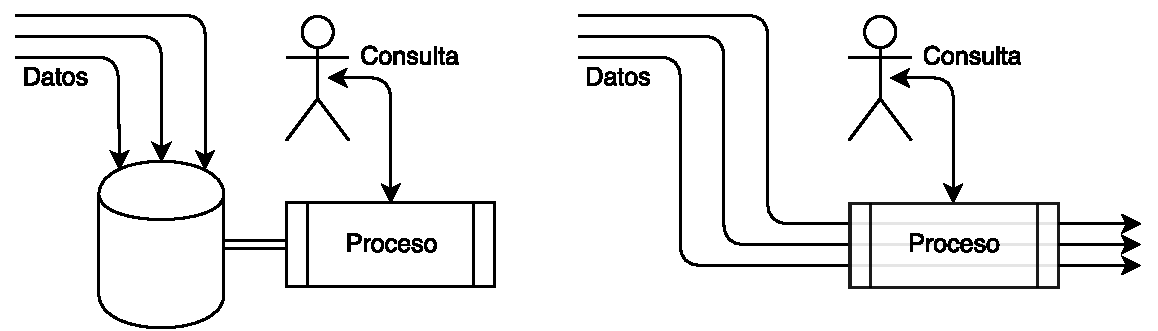
\includegraphics[width=0.8\textwidth]{./graph/bigdata_vs_streamingdata.pdf}
	\caption{Gráfica conceptual de BigData vs Streaming Data}
	\label{fig:bigdata_vs_streamingdata}
\end{figure}

En la figura \ref{fig:bigdata_vs_streamingdata} (izquierda) puede observarse un diagrama esquematizado del enfoque clásico de \textit{BigData}, donde todos los datos son almacenados en algún tipo de base de datos, y luego se realizan consultas sobre estos mediante algún proceso particular que permita extraer información relevante. A la derecha de la figura \ref{fig:bigdata_vs_streamingdata} se puede observar un esquema de las partes relevantes del enfoque de \textit{Data Streaming}; la diferencia más importante entre estos dos paradigmas es no existe la persistencia de datos. Las consultas se realizan sobre datos `en movimiento', en lugar de utilizar datos estáticos.

\

En los últimos años, los avances en las tecnologías de hardware han posibilitado colectar datos de forma continua. Transacciones que hacemos en nuestra vida cotidiana como el uso de una tarjeta de crédito, un teléfono o navegar la web generan grandes cantidades de datos. De la misma manera, los avances en las tecnologías de la información hicieron que los flujos de información en las redes IP sean cada vez mayores. En muchos casos, los datos generados pueden ser minados para obtener información relevante que puede ser utilizada en gran cantidad de aplicaciones. Sin embargo, cuando el volumen de datos es muy grande, se presentan algunos problemas:

\begin{itemize}
	\item No es posible un procesamiento eficiente de los datos usando métodos que requieran varias pasadas sobre el \textit{dataset} (por ejemplo, aquellos usados en \textit{BigData}). En su lugar, dada la velocidad a la que se producen estos datos, uno puede permitirse procesar cada dato a lo sumo una vez, lo que impone ciertas restricciones en la implementación de los algoritmos de procesamiento. Por lo tanto, las técnicas de procesamiento de \textit{Streaming Data} deben ser diseñadas de forma que los algoritmos cumplan su cometido con una única pasada por el conjunto de datos.
	\item En muchos casos, el proceso de minar \textit{Streaming Data} tiene una componente temporal inherente: los datos puede evolucionar a medida que pasa el tiempo. Este comportamiento de los \textit{streams} de datos es llamado \textit{localidad temporal}\cite{Aggarwal:2006:DSM:1196418}. Por esta razón, una adaptación directa de los algoritmos de una pasada para minar \textit{Streaming Data} puede no se una solución efectiva para esta tarea. Estos deben diseñados cuidadosamente haciendo foco en la evolución de los datos que están siendo procesados.
\end{itemize}

Antes de presentar algunas de las técnica existentes para procesar \textit{streams} de datos, es conveniente introducir la notación que utilizada para describirlos.

\subsection{El modelo de Data Streaming}
En el modelo de \textit{Data Streaming}, los datos que van a ser procesados no están disponibles para ser accedidas aleatoriamente desde disco o memoria, sino que llegan como uno o mas flujos continuos de datos. Los \textit{streams} de datos son diferentes de los modelos relacionales convencionales en varios aspectos: 
\begin{itemize}
	\item Los elementos del \textit{stream} deben ser procesados de manera \textit{online}, esto es, sin ser persistidos en ningún soporte de almacenamiento.
	\item Los sistemas que procesan los datos no tienen control sobre el orden en los elementos de la entrada.
	\item Los \textit{stream} de datos pueden ser infinitos.
	\item Una vez que un elemento es procesado, este se descarta.\footnote{En algunas aplicaciones los elementos pueden ser almanacenados para procesamiento posterior, pero en un modelo de \textit{streaming} "puro" los elementos son procesados una única vez.}
\end{itemize}

Otra característica de este modelo que es conveniente remarcar se relaciona con las consultas a los datos procesados: podemos hacer una distinción entre \textit{consultas únicas} y \textit{consultas continuas}\cite{Terry:1992:CQO:141484.130333}. Las primeras (como aquellas que se hacen mediante un DBMS tradicional) son evaluadas una vez sobre un conjunto de datos en un instante de tiempo particular (los datos no cambian durante la duración de la consulta). La consultas continuas, por otro lado, son evaluadas continuamente mientras el \textit{stream} de datos esta ocurriendo. Las respuestas a estas consultas pueden ser almacenadas y actualizadas en la medida que llegan nuevos flujos de datos, o pueden ser origen de otro \textit{stream} de datos.

\

Existen tres modelos diferentes para describir \textit{Streaming Data}. Supongamos que se quiere analizar un \textit{stream} de datos que está siendo generado por cierta aplicación. Los datos $t_1, t_2, \dots$ llegan secuencialmente, elemento por elemento, y describe una señal $\mathbf{a}$ como una función unidimensional $\mathbf{a}: [1 \dots N] \rightarrow R$. Los modelos difieren en cómo los $t_i$ describen a la señal $\mathbf{a}$.

\subsubsection{Modelo de series de tiempo}
Dado los elementos $t_i$ que se presentan en orden creciente de $i$, la señal $\mathbf{a}$ esta conformada por $\mathbf{a}[i]=t_i$. Este modelo es adecuado para ser usado cuando los elementos del \textit{stream} forman series de tiempo. Por ejemplo, si se quiere realizar observaciones sobre el volumen de transacciones del NASDAQ cada minuto.
\subsubsection{Modelo de caja registradora}
En este modelo, los $t_i$ modifican el estado de los $\textbf{a}[j]$. Podemos pensar cada elemento $t_i$ como una tupla $t_i = (j, I_i)$, $I_i \geq 0$ que provoca una actualización $\textbf{a}_i[j] = \textbf{a}_{i-1} [j] + I_i$ donde $\textbf{a}_i$ es el estado de la señal luego de procesar el i-ésimo elemento del \textit{stream}. Es importante observar que múltiples $t_i$ pueden incrementar un $\textbf{a}[j]$ a lo largo del tiempo. Este es tal vez el más popular de los modelos de \textit{streams} de datos. Es útil para aplicaciones como monitoreo de direcciones IP que acceden un servidor, direcciones IP de origen que envían paquete en un enlace dado, etc, dado que la misma dirección IP puede acceder al servidor muchas veces o puede enviar multiples paquetes en un período de tiempo dado.
\subsubsection{El modelo Turnstile}
De la misma forma que en el modelo anterior, los $t_i$ actualizan a los $\textbf{a}[j]$. Cada elemento $t_i = (j, U_i)$ produce  $\textbf{a}_i[j] = \textbf{a}_{i-1} [j] + U_i$ donde $\textbf{a}_i$ es la señal luego de la ocurrencia del i-ésimo elemento en el \textit{stream}, y $U_i$ puede ser positivo o negativo. Este modelo es el mas general de todos (notar que es igual al modelo de caja registradora, pero admite valores de $I_i$ negativos). Es apropiado para estudiar situaciones completamente dinámicas donde puede haber inserción y borrado de elementos. 

\

Realizar consultas sobre \textit{streams} de datos presenta desafíos únicos. Dado que los flujos de datos son potencialmente infinitos, la cantidad de espacio de almacenamiento requerido para calcular la respuesta exacta de una consulta acerca de los datos también podría crecer infinitamente. Si bien se han estudiado algoritmos para procesar conjuntos de datos que exceden la memoria principal de una computadora\cite{Vitter:2001:EMA:384192.384193}, estos no son útiles para aplicaciones de \textit{Data Streaming} dado que no soportan consultas continuas y son típicamente muy lentos para generar resultados en tiempo real. El modelo en discusión es aplicable a problemas donde es importante que los resultados de las consultas realizadas se obtengan rápidamente y donde hay grandes volúmenes de datos que están siendo producidos continuamente a gran velocidad. Nuevos datos continúan llegando mientras los datos previos están siendo procesados; el tiempo de cómputo por dato debe ser bajo, de lo contrario, se introduce latencia y el algoritmo no será capaz de procesar los datos en tiempo real. Por este motivo, estos algoritmos deben ser capaces de funcionar haciendo uso únicamente de la memoria principal, sin realizar accesos a disco.

Cuando la cantidad de memoria disponible es finita, no siempre es posible producir respuestas exactas a las consultas realizadas a \textit{streams} de datos (recordemos, potencialmente de duración infinita). Sin embargo, es posible obtener muy buenas aproximaciones a las mismas, que son aceptables cuando no se dispone de la respuesta exacta. Si bien distintos algoritmos para aproximar respuestas a consultas realizadas sobre \textit{streams} de datos han sido estudiados en los últimos años, para este trabajo haremos foco en una estructura de datos conocida como  \textit{sketch}\cite{Alon:1996:SCA:237814.237823}\cite{Flajolet:1985:PCA:5212.5215} debido a las bondades que presentan. Además, introduciremos algunas técnicas de conteo de gran utilidad para resolver ciertos problemas de minado de \textit{Streaming Data}.


\newpage

\section{El problema de los elementos frecuentes}
El problema de los elementos frecuentes es uno de los más estudiados desde los años 80 dada su importancia en el minado de \textit{Data Streams}. Muchas de las técnica utilizadas en este área se basan directa o indirectamente en encontrar elementos frecuentes en \textit{streams} de datos. Enunciado de forma sencilla, el problema consta en determinar aquellos elementos que tienen mayor frecuencia de ocurrencia dado un \textit{stream} de elementos. Aquí asumimos que el \textit{stream} es lo suficientemente largo como para que las soluciones convencionales, intensivas en uso de recursos, como ordenar los elementos o mantener un contador por cada uno estos, sean inviables. 
\

Podemos dividir los algoritmos para encontrar elementos frecuentes en tres clases. Los \textbf{algoritmos basados en conteo} operan sobre un subconjunto de elementos y mantienen un contador asociado a los mismos. Por cada entrada nueva, el algoritmo decide si actualizar o no el contador del elemento, y de hacerlo, con que valor lo afecta. 
La segunda clase de algoritmos, que no será analizada en este documento, es una derivación de los \textbf{algoritmos de cuantiles}; el problema de encontrar cuantiles en la distribución de un \textit{stream} de datos nos permite encontrar elementos frecuentes.
Finalmente, los algoritmos basados en \textbf{\textit{sketches}} utilizan proyecciones lineales aleatorias de las entradas\cite{Cormode:2008:FFI:1454159.1454225} (vistas como vectores de características) y por lo tanto, no almacenan explícitamente los elementos de entrada. Estos últimos tienen ciertas propiedades que son de gran utilidad para procesamiento de múltiples \textit{streams} de datos.

\subsection{Elementos frecuentes en data streams}\label{elementos_frecuentes_en_datastreams}
Antes de describir los algoritmos para encontrar elementos frecuentes es necesario enunciar formalmente el problema.

\subsubsection{Elementos frecuentes}\label{elementos_frecuentes} Dado un stream $S$ de $n$ elementos $t_1$, $t_2$, \dots, $t_n$, la frecuencia del elemento $i$ es $f_i = |\{j|t_j=i\}|$ (es decir, la cantidad de índices $j$ donde el $j$th elemento es $i$). Los $\phi$ elementos frecuentes están dados por $\{i|f_i>\phi n\}$.

\textbf{Ejemplo}: El stream $S=\{a,a,b,a,c,b,a\}$ tiene $f_a=4$, $f_b=2$ y $f_c=1$. Para $\phi=0.2$ los elementos frecuentes son $a$ y $b$.

\

Encontrar exactamente los $\phi$ elementos frecuentes puede ser costoso en términos de recursos: un algoritmo que resuelve el problema de los elementos frecuentes debe usar una cantidad lineal de espacio\cite{Cormode:2010:MFF:1731351.1731356}. Para relajar el requerimiento de recursos se utiliza una aproximación a la solución del problema.

\subsubsection{$\epsilon$-aproximación de elementos frecuentes} 
Dado un stream $S$ de $n$ elementos una $\epsilon$-aproximación de los elementos frecuentes esta dada por el conjunto $F$ tal que todos los elementos $i \in F$ tengan frecuencia $f_i > (\phi - \epsilon)n$, y que no exista $i \notin F$ con $f_i > \phi n$. Dicho de otra manera, una $\epsilon$-aproximación de los elementos frecuentes consiste en encontrar todos los elementos con frecuencia mayor o igual a $\phi n$, de los cuales ninguno tiene frecuencia menor que $(\phi - \epsilon) n$.

\subsubsection{Estimación de la frecuencia de un elemento}
Un problema relacionado a los anteriores consiste en estimar la frecuencia de los elementos al momento que se están procesando los datos. Dado un stream $S$ de $n$ elementos con frecuencias $f_i$, el problema de estimación de frecuencia consiste en procesar el stream de forma que para cualquier $i$ se pude obtener un $\hat{f_i}$ tal que $\hat{f_i} \leq f_i \leq \hat{f_i}+\epsilon n$.

\

Los elementos frecuentes, también llamados \textbf{heavy hitters}, son problemas muy estudiados por sus aplicaciones en bases de datos y \textit{data streaming}. Son también conocidos como \textit{top-k}, \textit{frequent items}, \textit{elephants} o \textit{iceberg queries}. Usualmente, cuando se busca identificar estos elementos de forma \textit{on-line} se trabaja en ventanas de tiempo acotadas o épocas de detección con el objetivo de encontrar \textit{heavy hitters} en momentos particulares del tiempo. Otro patrón que resulta de interés para caracterizar los datos en tránsito son los \textbf{heavy changers}: podemos decir que los \textit{heavy changers} son aquellos elementos que varían de forma significativa en épocas consecutivas, es decir, presentan inconsistencias significativas entre el comportamiento observado y el comportamiento normal del flujo de datos (el cual se basa en lo ocurrido en el pasado) en un período de tiempo acotado\cite{Tong:2016:HTS:2927964.2927977}.

\begin{center}
	\rule{4in}{0.3pt}
\end{center}

\subsection{Elementos frecuentes: un escenario de aplicación}
Los dispositivos conectados a Internet y a grandes redes privadas transfieren paquetes IP. Para manejar estas redes es necesario entender en existencia de fallas, la ocurrencia de ciertos patrones de uso y actividades poco usuales en progreso. Esto hace necesario el análisis del tráfico y fallas en tiempo real.

Consideremos el trafico de datos en redes TCP/IP. Este puede ser visto en varios niveles:
\begin{itemize}
	\item En el nivel más granular tenemos logs de capa de red: cada paquete IP tiene una cabecera que contiene dirección IP de origen y destino, puertos, etc.
	\item En un nivel más de agregación tenemos los logs de flujos: cada flujo es una colección de paquetes con el mismo valor para cierto atributo, como la dirección IP de origen y destino, y el log contiene información acumulada del número de bytes y paquetes enviados, tiempo de comienzo y fin de la transmisión, protocolo, etc.
	\item Al nivel más alto, tenemos logs SNMP, que son los datos agregados del número de bytes enviados a través de cada nodo cada cierta cantidad de minutos.
\end{itemize}

Si bien procesar datos agregados no demanda el uso de recursos computacionales de forma intensiva, utilizar información de mas bajo nivel nos permite tenes más precisión en los resultados de los algoritmos dado que estamos procesando mayor cantidad de información, lo que representa de mejor manera la realidad. Por ejemplo, podemos pensar a los segmentos TCP que pasan por un \textit{gateway} como los elementos de un \textit{stream} de datos. Aunque estos ocurren de manera secuencial, pertenecen a diferentes sesiones que están activas al mismo tiempo. De esta manera se puede analizar el comportamiento del tráfico de red de todas las sesiones en búsqueda de elementos frecuentes.

Consideremos el problema de determinar la frecuencia de ocurrencia de cierto evento, perteneciente a algún universo de eventos posibles $U$. Para obtenerla basta con llevar registro de la frecuencia $f_i$ por cada elemento $i \in U$: dado $U_0=\{a,b,c\}$ y una serie o stream de eventos $S=\{a,a,b,a,c,b,a\}$, la frecuencia de ocurrencia de cada elemento de $U_0$ es $f_a=4$, $f_b=2$ y $f_c=1$.  A pesar de su simpleza, el costo de memoria de este algoritmo crece exponencialmente cuando la cantidad de eventos posibles $|U|$ aumenta. En términos de implementación, el $|U|$ esta dado por la cantidad de bits que se usen para representar el conjunto. Así, si usamos contadores de 32 bits y $|U|=2^{16}$ tenemos que se necesita almacenar en memoria $2^{16} * 32 \ bits\equiv 8$ KB en contadores, uno por cada evento posible de $U$. 

\begin{figure}[ht]
	\centering
	\begin{tikzpicture}
	\begin{axis}[
	axis lines = left,
	xlabel = $x$,
	ylabel = {$f(x)$},
	xlabel={Cantidad de bits para representar los elementos de $U$},
	ylabel={Uso de memoria en GB},
	xtick={0,4,8,12,16,20,24,28,32,36},
	ymajorgrids=true,
	xmajorgrids=true
	]
	\addplot [
	domain=0:37, 
	samples=100, 
	color=red
	]
	{(2 ^ x *32)/ (1024 ^ 3)};
	\end{axis}

	\end{tikzpicture}

	\caption{Uso de memoria en función del tamaño del universo de elementos posibles.}
	\label{fig:universe_exponencial}
\end{figure}

Sin embargo, como podemos ver en la figura \ref{fig:universe_exponencial}, el uso de memoria crece exponencialmente a medida que nuestro universo de posibles elementos se hace más grande.
Este tipo de problemas y similares llevaron al desarrollo de diferentes técnicas de conteo: bajo esta abstracción, los algoritmos procesan la entrada una única vez y deben calcular de manera precisa varios resultados usando recursos (espacio y tiempo por elemento) de forma estrictamente sublineal al tamaño de la entrada\cite{Muthukrishnan:2005:DSA:1166409.1166410}. Existen diferentes algoritmos para procesar y obtener información acerca de los eventos usando estructuras de datos que utilizan el espacio de memoria eficientemente. Sin embargo, estos métodos no calculan la frecuencia exacta de cada evento sino que la estiman: en general, para cantidades masivas de eventos basta con tener una buena aproximación de las frecuencias para identificar anomalías.

\newpage

\section{Técnicas para encontrar elementos frecuentes}\label{sec:tecnicas_elementos_frecuentes}
En algunos escenarios, resolver exactamente el problema de los $phi$ elementos frecuentes que se enunció en la sección \ref{elementos_frecuentes} es inviable dado a los requerimientos de espacio que presenta\cite{Charikar:2002:FFI:646255.684566}. Se han propuesto gran variedad de algoritmos para la resolución del mismo y sus variaciones \cite{Charikar:2002:FFI:646255.684566}\cite{Cormode:2005:WHW:1061318.1061325}\cite{Demaine:2002:FEI:647912.740658}\cite{Manku:2002:AFC:1287369.1287400}. Cómo se mencionó anteriormente, esta técnicas pueden ser clasificas en dos tipos, que se describen a continuación.

\subsection{Técnicas basadas en conteo}\label{tecnicas_conteo}

Los algoritmos basados en técnicas de conteo mantienen contadores para un subconjunto $T$ del universo de elementos posibles $U$. A continuación se describen algunos algoritmos de conteo existentes y sus características.

\subsubsection{MAJORITY}
El problema de los elementos frecuentes fue estudiado por primera vez en la década del 80, y fue enunciado de esta manera:
\begin{displayquote}
	Supongamos una lista de $n$ números, representando los "votos" de $n$ procesadores en el resultado de cierto cálculo. Queremos determinar si hay un voto mayoritario y cual es ese voto.\cite{GUIBAS1981208}
\end{displayquote}

Para solucionar el problema, los autores desarrollaron un algoritmo de una pasada llamado MAJORITY. Este puede ser descrito de la siguiente manera: se inicializa una elemento cualquiera con su contador en $0$. Por cada elemento subsecuente del \textit{stream}, si es el mismo que el elemento almacenado, se incrementa el contador en $1$. Si el elemento es diferente y el contador es $0$, entonces se reemplaza el elemento y se incrementa el contador en $1$. De lo contrario, se decrementa el contador. Luego de procesar todos los elementos, el algoritmo garantiza que si hay un voto mayoritario, entonces este debe ser presentado por el algoritmo. En el peor caso, si se procesa un \textit{stream} de $n$ elementos, el algoritmo realiza $2n$ comparaciones.

Sea cada elemento $t_i = (j, I_i)$ con $I_i = 1$, el pseudocódigo de MAJORITY es como sigue:

\begin{algorithm}
	\SetKwInOut{Input}{Input}
	\SetKwInOut{Output}{Output}
	
	\underline{function MAJORITY} $()$\;
	\Input{Un \textit{stream} de elementos $t_i \in S$}
	\Output{El elemento con mayor frecuencia de ocurrencia}
	$e \leftarrow \emptyset$\; $c \leftarrow 0$\;
	\ForEach{$t_i$}
	{
		\eIf{$j=e$}
		{
			$c \leftarrow c + 1$\;
		}{
			\eIf{$c=0$}{
				$e \leftarrow j$\;
				$c \leftarrow 1$\;
			}{
				$c \leftarrow c - 1$\;
			}
		}
	}
	\caption{Algoritmo MAJORITY para encontrar el elemento mas frecuente}
	\label{alg:majority}
\end{algorithm}

Usando un argumento de paridad podemos concluir que el resultado del algoritmo es el correcto: si por cada elemento que no es el mayoritario tomamos uno de los mayoritarios, al final van a quedar solo elementos del conjunto mayoritario.
\
Como puede observarse en el algoritmo \ref{alg:majority} no existe valor de retorno. En general, los algoritmos para procesar \textit{streams} de datos actualizan su estado con cada elemento procesado, evitando retornar valor alguno e interrumpir su ejecución. Esto es característico de los algoritmos de \textit{Data Streaming} dado que se suponen \textit{streams} de datos infinitos.

\subsubsection{FREQUENT}\label{FREQUENT}

Este algoritmo, que es una generalización de MAJORITY, fue presentado simultáneamente en \cite{Karp:2003:SAF:762471.762473} y \cite{Demaine:2002:FEI:647912.740658}. Permite encontrar todos los elementos en el \textit{stream} de datos cuya frecuencia excede cierto umbral $\phi = 1/(k+1)$ dado un $k \in Z$. 

\paragraph{Teorema} Existe un algoritmo de una pasada que usa $k$ contadores y puede determinar un conjunto de a lo sumo $k$ elementos incluyendo aquellos que ocurren más de $N/(k+1)$ veces en un \textit{stream} de elementos de longitud $N$.


\paragraph{Prueba} Sea un elemento $x$ que ocurre $t > N/(k+1)$ veces. Supongamos que $x$ fue visto $t_f$ veces cuando los $k$ elementos ya estaban siendo usados con otros elementos distintos de $x$, y $t_i$ veces cuando aún existía lugar para agregar su contador o este estaba siendo usado. Así, el contador de $x$ se incrementa $t_i$ veces, y $t_f + t_i = t > N/(k+1)$. Además, sea $t_d$ el número de veces que el contador de $x$ es decrementado dada la ocurrencia de un elemento distinto de $x$. Dado que un contador nunca es negativo, $t_i \geq t_d$. Si la desigualdad es estricta, $x$ es siempre positivo cuando el algoritmo termina.
Con cada uno de los $t_f + t_d$ decrementos, podemos inferir la ocurrencia de otros $k$ elementos, además de $x$. Así, $(k+1)(t_f + t_d) \leq N$. Si el valor final de $x$ es $0$, entonces $t_d = t_i$, y por lo tanto $t = t_f + t_i = t_f + t_d > N/(k+1)$. Multiplicando a ambos lados por $(k+1)$, que es siempre positivo,  tenemos $(m+1)(t_f + t_d) > N$ que es una contradicción. Finalmente, concluimos que $t_i > t_d$, por lo que el contador de $x$ permanece positivo y $x$ es al menos uno de lo $k$ candidatos restantes. \textbf{*}

\

Dada una secuencia elementos $S = \{t_1, t_2, ..., t_N\}$ y un universo $U$ de elementos posibles, tal que $t_i \in U$, $|U| = n$, $\phi \in R$ y $0 < \phi < 1$. Suponemos ademas que $N \gg n \gg k$. Queremos encontrar el conjunto $H \subset U$ cuyos elementos tengan una frecuencia de ocurrencia mayor a $\phi N$, esto es, aquellos elementos $e \in H$ tal que $f_H(e) > \phi N$ donde $f_H(x)$ es el número de ocurrencias $\forall x \in S$. 

En lugar de guardar solo un elemento y un contador FREQUENT almacena una lista $\mathbf{A}$ de $l$ elementos (es implementado mediante un diccionario), cada uno con un contador asociado tal que $|\mathbf{A}| \equiv |H|$. Cada nuevo elemento es comparado contra los elementos existentes en $\mathbf{A}$ y se incrementa el contador correspondiente. Si el elemento no está presente en la lista puede suceder lo siguiente: si algún contador está en cero se reemplaza el elemento asociado y se inicializa el contador en $1$. Si los contadores de todos los elementos están siendo utilizados, entonces todos son decrementados en $1$. Este algoritmo asegura que, al finalizar su ejecución, cada contador asociado a cada elemento esta a lo sumo $\epsilon N$ unidades por debajo del valor real si $k = 1/ \epsilon$.\cite{Kranakis03boundsfor}.


\

\begin{algorithm}
	\SetKwInOut{Input}{Input}
	\SetKwInOut{Output}{Output}
	
	\underline{function FREQUENT} $(l, k)$\;
	\Input{Un \textit{stream} de elementos $t_i \in S$}
	\Output{Los elementos cuya frecuencia excede $1/k$}
	$n \leftarrow 0$\;
	$A \leftarrow \emptyset$\;
	\ForEach{$t_i$}
	{
		$n \leftarrow n + 1$\;
		\eIf{$t_i \in A$}
		{
			$A[t_i] \leftarrow A[t_i] + 1$\;
		}{
			\eIf{$|A| < l$}{
				$A[t_i] \leftarrow 1$\;
			}{
				\ForAll{$t_j \in A$}
				{
					$A[t_j] \leftarrow A[t_j] - 1$\;
					\If{$A[t_j] \leq 0$}{$A[t_j] \leftarrow \emptyset$}
				}
			}
		}
	}
	\caption{Algoritmo FREQUENT para encontrar los $k$-elementos frecuentes}
	\label{alg:frequent}
\end{algorithm}

FREQUENT puede resolver el problema de estimación de frecuencia desarrollado en la sección \ref{elementos_frecuentes} con $\epsilon = 1/k$. El algoritmo $O(n)$ en tiempo y $O(1)$ en memoria.

\subsection{Técnicas basadas en sketches}

Muchas técnicas desarrolladas para procesar grandes volúmenes de datos y realizar consultas sobre los mismos asumen que los datos son estáticos, almacenados en algún soporte físico. Sin embargo, para ciertas aplicaciones este enfoque no es viable. Esta restricción es la que más importancia tuvo en relación al nacimiento de los métodos de \textit{data streaming} e impulso el desarrollo de algoritmos livianos sumamente eficientes (sublineales en el uso de memoria), y estructura de datos probabilistas que pueden usarse para responder ciertas preguntas sobre los datos, de manera precisa y con una probabilidad razonablemente alta. Este nuevo enfoque utiliza una representación comprimida (con cierta pérdida) de los datos en lugar de almacenarlos en su totalidad.

Los \textit{sketch} son estructuras de datos compactas, capaces de representar vectores de alta dimensionalidad y responder consultas realizadas sobre estos vectores con garantía de alta precisión en la respuesta\cite{Cormode:2005:IDS:1073713.1073718}. Son usadas en situaciones donde el costo de almacenar la totalidad de los datos es prohibitivo (al menos en soporte de acceso rápido como la memoria en contraposición de disco rígido). La estructura de datos mantiene una proyección lineal del vector junto con un conjunto de vectores aleatorios (definidos implícitamente por funciones simples de \textit{hash}). Al incrementar el rango de las funciones de \textit{hash} se incrementa la precisión de la representación, y al incrementar el número de funciones de \textit{hash} disminuye la probabilidad de realizar malas estimaciones.
Si representamos las entradas como vectores, estos pueden ser multiplicados por una \textit{matriz sketch}. El \textit{vector sketch} resultado contiene la  información suficiente para responder de forma aproximada ciertas preguntas sobre los datos procesados. Por ejemplo, si codificamos los elementos del \textit{stream} de datos como vectores cuya $i$-ésima entrada es su frecuencia $f_i$, el \textit{sketch} es el producto de este vector y una matriz\footnote{Existen diferentes formas de definir la \textit{matriz sketch}, cada una con aplicaciones particulares. Para conteo de eventos se usan familias de funciones de \textit{hash} con ciertas propiedades para definir la proyección lineal.}.

Los algoritmos basados en \textit{sketches} resuelven el problema de estimación de frecuencia descrito en \ref{elementos_frecuentes_en_datastreams}, pero necesitan información adicional para resolver el problema de los elementos frecuentes. Por esto, se suele aumentar la estructura de datos de los \textit{sketches} con algún método de conteo para estimar la frecuencia de los elementos de manera eficiente.

\

Dado que el funcionamiento de estas estructuras puede parecer contra intuitivo, es conveniente introducir una estructura de datos similar (especialmente en las variantes que realizan conteo de elementos) llamada filtro de \textit{Bloom}, de forma de ganar intuición acerca del funcionamientos de los \textit{sketches}.

\subsubsection{Filtros Bloom}

Un filtro de \textit{Bloom} es una estructura de datos probabilista, eficiente en uso de memoria, utilizada para determinar si un elemento pertenece o no a un conjunto o \textit{set}. La misma puede reportar falsos positivos cuando se consulta por la existencia de cierto elemento al conjunto\cite{Putze:2010:CHS:1498698.1594230}; en otras palabras, una consulta puede retornar que es \textit{posible que el elemento sea parte del conjunto} o que \textit{definitivamente no esta presente en el conjunto}. La ventana principal de esta estructura de datos sobre las tradicionales es la eficiencia en el uso de memoria.


Para representar un conjunto $U$ de $n$ elementos posibles, un \textit{filtro Bloom} clásico hace uso de un vector de $m$ bits con $m \ll n$. Al comienzo todos los bits están en $0$. Deben existir un conjunto de $k$ funciones de hash diferentes, las cuales mapean elementos del conjunto $U$ a una de las $m$ posiciones del vector: $h_i(e): U \rightarrow m$, $e \in U$, $m \in \mathbf{Z}$ y $0 < i < k$.


Para insertar un elemento $e$ en el filtro se calcula las posiciones en el array evaluando las $k$ funciones de hash $h_1(e)$, $h_2(e)$, \dots, $h_k(e)$. Luego se asigna un $1$ a cada posición del array. Para consultar si un elemento $e'$ está presente o no en el conjunto se deben evaluar las $k$ funciones de hash $h_1(e')$, $h_2(e')$, \dots, $h_k(e')$ para obtener $k$ posiciones en el filtro. Si al menos un bit de los apuntados por las funciones de hash es $0$, entonces el elemento $e'$ no existe en el conjunto. Si todos los bits que indican las funciones de hash están en $1$ es probable que el elemento sea parte del conjunto.

\begin{figure}[ht]
	\centering
	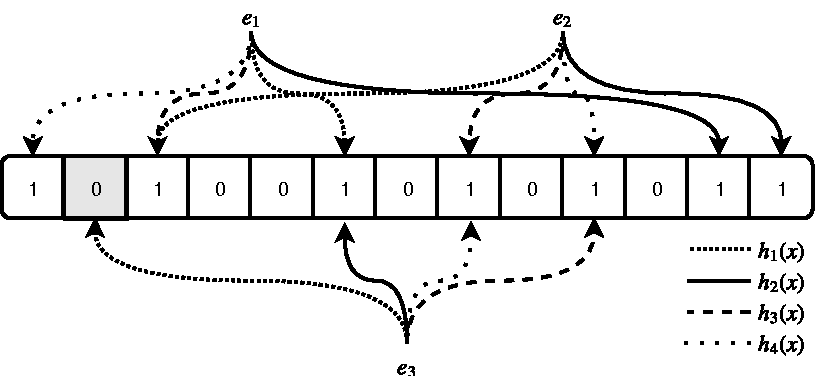
\includegraphics[width=1\textwidth]{./graph/bloom.pdf}
	\caption{Filtro Bloom}
	\label{fig:bloom}
	\medskip
	\small
	
	\parbox{13.1cm}{La imagen muestra un filtro de Bloom luego que los elementos $e_1$ y $e_2$ fueron insertados. El elemento $e_3$ no se encuentra en el conjunto dado que al menos uno de los bits a los que apuntan las funciones de hash es $0$. La pertenencia de un elemento $e'$ al conjunto puede ser reportada erróneamente si las $k$ funciones de hash $h_i(e')$ apuntan a bits con valor $1$.}
	
\end{figure}

La ventaja principal de los filtros de \textit{Bloom} es evidente cuando se la compara con otras estructuras de datos usadas para implementar \textit{sets} (listas, tablas de \textit{hash}, arboles binarios de búsqueda, etc). Estas requieren almacenar el elemento en sí, lo cual puede requerir una cantidad pequeña de bits si los elementos son números enteros, hasta un número arbitrario de bits en el caso que los elementos sean \textit{strings}. Sin embargo, estas estructuras probabilísticas no necesitan almacenar el elemento en sí, y tampoco introducen el \textit{overhead} generado por los punteros que utilizan las estructuras enlazadas como las listas.

La cantidad óptima de funciones de hash $k$ puede deducirse como sigue. Sea la probabilidad que uno de los bits del filtro de \textit{Bloom} sea 0:

\begin{equation}
	\mathcal{P} [h_i(x)=0 ] = (1- \frac{1}{m})^{kn} \approx e ^ {-\frac{kn}{m}} = p
\end{equation}

La probabilidad de tener un falso positivo está dada por:
\begin{equation}
	(1 - e ^ {-\frac{kn}{m}})^k = (1 - p)^k = \varepsilon
\end{equation}

El valor óptimo de $\hat{k}$ se obtiene al minimizar la ecuación anterior, de forma que $\hat{k} = \ln(2) \frac{m}{n}$. La probabilidad de falso positivo está dada por la fórmula\cite{Bloom:1970:STH:362686.362692}:
\begin{equation}
	\varepsilon = (0.5) ^ {\hat{k}} = (0.6185)^{\frac{m}{n}}
\end{equation}

Un filtro de \textit{Bloom} con un error de $1\%$ y un valor óptimo de $k$ requiere alrededor de $10$ bits por elemento, sin importar el tamaño del elemento. Para reducir el error a un $0.1\%$ se deben emplear alrededor de $15$ bits.

\

Esta estructura de datos, en su versión clásica, no resuelve el problema de los elementos frecuentes (para esto se utiliza una variante llamada \textit{filtros de conteo}). Sin embargo, resulta útil para ganar intuición: los algoritmos de \textit{sketches} son similares a los filtros de \textit{Bloom} en el uso de las funciones de hash para representar conjuntos de elementos. Utiliza estructuras auxiliares que permiten aproximar el número de elementos que fueron vistos en el \textit{stream} de datos.  

\subsubsection{CountMin Sketch}

Los \textit{sketches} son menos conocidos que los filtros \textit{Bloom} pero comparten ciertas similitudes. Son estructuras de datos que permiten sumarizar un \textit{stream} de datos y pueden utilizarse para resolver el problema de los elementos frecuentes. Esto puede ser llevado a cabo usando menos espacio del que se utilizaría almacenando un contador por elemento, pero permitiendo que los contadores tengan cierto error en algunas ocasiones. Si bien existen otras implementaciones cómo Count Sketch\cite{Charikar:2002:FFI:646255.684566} y AMS Sketch\cite{Alon:1996:SCA:237814.237823}, CountMin Sketch es una estructura de datos mas sencilla, fácil de construir, que asegura muy buenas garantías de precisión cuando se hacen consultas sobre los datos procesados.

Un CM Sketch es simplemente una matriz de contadores de $d$ filas y $w$ columnas, cuyo valor inicial es $0$. Además, se escogen aleatoriamente $d$ funciones de hash de una familia de funciones de hash independientes de a pares (ver Sección \ref{k_independent_hash_func}):
\begin{equation*}
	h_1 \dots h_d: \{1 \dots n\} \rightarrow \{1 \dots w\}
\end{equation*}

Una vez que $w$ y $d$ son definidos, el espacio alocado no varía: la estructura de datos es representada por $wd$ contadores y $d$ funciones de hash (que puede ser representado en $O(1)$ variables\cite{Motwani:1995:RA:211390}).


Sea $\mathbf{a}$ un vector de dimensión $n$ cuyo estado en el tiempo $t$ es $\mathbf{a}(t)=[a_1(t), a_2(t), \dots, a_n(t)]$. Inicialmente $\mathbf{a}$ es el vector $\mathbf{0}$, es decir $a_i(0)=0 \ \forall i$. Las actualizaciones a los elementos de $\mathbf{a}$ se representan mediante un \textit{stream} de tuplas. De forma general, la tupla $(i_t, c_t)$ representa el $t$-ésimo elemento procesado\footnote{Para conteo de elementos $c_t=1$.}:

\begin{gather*}
a_{i_t}(t)=a_{i_t}(t-1) + c_t\\
a_{i_{t'}}(t)=a_{i_{t'}}(t-1) \ \forall t' \neq t 
\end{gather*}

Por cada elemento del \textit{stream} se calculan las $d$ posiciones de los contadores mediante $(j, h_j(i_t))$ para $j \in \{0,1 \dots d-1 \}$ y se los actualiza con el valor de $c_t$:

\begin{figure}[ht]
	\centering
	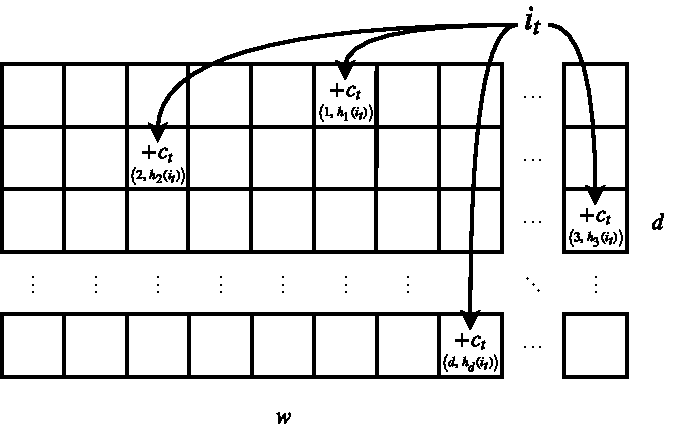
\includegraphics[width=1\textwidth]{./graph/cm_sketch.pdf}
	\caption{COUNTMIN Sketch}
	\label{fig:cm_sketch}
	\medskip
	\small
	
	\parbox{13.1cm}{La figura muestra el proceso de actualización de un sketch COUNTMIN. Se calcula la posición de los contadores para cada fila evaluando la función de hash correspondiente con el elemento $i_t$. Luego, los contadores de las posiciones $(j, h_j(i_t))$ se actualizan con el valor de $c_t$.}
	
\end{figure}

Formalmente, dado $(i_t, c_t)$, se realizan las siguientes modificaciones:
\begin{equation}
	\forall \ 0 \leq j < d: CM[j, h_j(i_t)] \leftarrow  CM[j, h_j(i_t)] + c_t
\end{equation}

Como computar cada función de hash es $O(1)$, el proceso completo de actualización es $O(d)$ (independiente de $w$). Por este motivo, esta estructura de datos es ideal para procesar datos que son generados a gran velocidad.

Los sketches pueden ser usados para estimar el valor de $a_i$ en cualquier instante de tiempo. El proceso de consulta es similar al de actualización: dado un $i_t$, podemos estimar el valor $a_i$ de la siguiente forma:

\begin{equation}
	\hat{a}_i = \min_{\{0,1  \dots d-1 \}}CM[j, h_j(i_t)]
\end{equation}

\paragraph{Teorema} Sea $w=\lceil e / \varepsilon \rceil$ y $d=\lceil \ln (1 / \delta) \rceil$, la estimación $\hat{a}_i$ tiene las siguientes garantías: $a_i \leq \hat{a}_i$ y, con probabilidad al menos $1-\delta$:
\begin{equation}
	\hat{a}_i = a_i + \varepsilon ||\mathbf{a}||_1
\end{equation}
El desarrollo y la demostración de este teorema puede encontrarse en \cite{Cormode:2005:IDS:1073713.1073718}. Es importante remarcar cómo se comporta la estimación de los contadores cuando variamos el tamaño de la matriz. A medida que agregamos filas, el valor de $\delta$ tiene que disminuir, por lo que la probabilidad que $\hat{a}_i$ este acotado como se muestra en el teorema aumenta. Además, cuando la cantidad de columnas $w$ aumenta, el valor de $\varepsilon$ tiene que disminuir, haciendo que la estimación $\hat{a}_i$ se aproxime cada vez más a el valor real.

\subsection{Estructura de datos propuesta}
A lo largo de los años, la comunidad ha estudiado y publicado numerosas mejoras a estas estructuras de datos. En particular, los LD-Sketch \cite{Huang:2015:HLD:2839515.2839568} hacen uso de las técnicas de conteo tratadas en \ref{tecnicas_conteo}, mejorando así la precisión de las estimaciones. Además, sus autores proponen una arquitecta donde cada objeto puede ser almacenado y actualizado de forma distribuida, permitiendo procesar un conjunto de sketches en paralelo, brindando redundancia y la posibilidad de escalar el sistema para hacer frente a volúmenes masivos de datos.

La idea principal es hacer que cada celda del sketch utilice una técnica de conteo para mantener conjunto de potenciales elementos anómalos en una lista asociativa. La detección local\footnote{Únicamente se trabajará con detección local. La detección distribuida reduce la cantidad de falsos positivos combinando los resultados de varios sketches procesados en paralelo.} garantiza la ausencia de falsos negativos y permite identificar elementos anómalos (con algunos falsos positivos) en un único nodo de cómputo.

Para la técnica de conteo FREQUENT (ver \ref{FREQUENT}) el siguiente lema muestra la cota de error para el valor estimado\cite{Misra1982143}.

\paragraph{Lema 1} Sea un stream de datos $\{(j, I_i)\}$ con $I_i=1$, $S(x)$ representa la cantidad de elementos $x$ que ocurrieron en una época y $U$ todos los elementos procesados en esa época. Si $j$ se mantiene en $A$, entonces $A[j] \leq S(x) \leq A[j] + \frac{U}{l}$. Si $x$ no se mantiene en $A$, su valor estimado es $0$ y $0 \leq S(x) \leq \frac{U}{l}$

\

Las técnicas basadas en conteo pueden identificar todos los \textit{heavy hitters} (sin incurrir en falsos negativos) que excedan el umbral $\phi = \frac{U}{l}$ consultando los elementos de la lista asociativa.

Consideremos ahora un \textit{sketch} con $r$ filas. A cada fila $i$ ($1 \leq i \leq r$) se le asocian $w$ cubetas\footnote{La posición que define el valor de hash de un elemento suele referirse en la literatura como bucket} y una función de hash 2-universal independiente $f_i$ que mapea un elemento o \textit{key} a una de las $w$ cubetas. Hacemos referencia a la j-ésima cubeta ($1 \leq j \leq w$) de la fila $i$ usando ($i$,$j$). Cada cubeta tiene un contador $V_{i,j}$ que se inicializa en 0. Por cada elemento ($x$, $v_x$) en el \textit{stream} de datos, el proceso de actualización calcula el valor de hash de $x$ para cada una de las $r$ filas, incrementando el valor del contador en $v_x$ (como se mencionó anteriormente, $v_x=1$).

Las técnicas basadas en sketches pueden identificar todos los \textit{heavy hitters} (sin falsos negativos) cuyo valor exceda el umbral $\phi$ comprobando si la cubeta correspondiente de todas las $r$ filas tiene valores por encima de $\phi$. Para detectar \textit{heavy changers}, se debe computar la diferencia entre los contadores de cada cubeta en dos \textit{sketches} adyacentes en el tiempo. Por la propiedad lineal de los mismos, la diferencia de cada cubeta es también la suma de las diferencias de los elementos hasheados a la misma. Si un elemento difiere en más de $\phi$ en todas las cubetas correspondientes a las $r$ filas, este es reportado como \textit{heavy changer}.

\subsubsection{Construcción de las funciones de hash}

\subsubsection{Proceso de actualización}

Los \textit{sketches} implementados en este desarrollo (a los que referiremos como \textit{LP-Sketch}) están inspirados en los \textit{LD-Sketch} y usan de base la estructura de los \textit{CM-Sketch}: consisten en una matriz de contadores de $r$ filas y $w$ columnas donde en cada cubeta ($i,j$) se mantiene un contador $V_{i, j}$, pero además se agregan 3 componentes adicionales:
\begin{itemize}
	\item Un vector asociativo o diccionario $A_{i,j}$ usado para implementar uno de los métodos de detección basado en conteo descrito anteriormente.
	\item Una variable $l_{i,j}$ que define la longitud máxima del vector asociativo $A_{i,j}$.
	\item El error máximo de estimación de la suma real de los elementos cuyo hash apunta a la cubeta ($i,j$), que representado por $e_{i,j}$.
\end{itemize}

El vector $A_{i,j}$ es usado para mantener el conjunto de \textit{heavy keys} candidatos en la cubeta ($i,j$). Por lo tanto, en el procedimiento de detección solo inspeccionamos los \textit{heavy keys} candidatos almacenados solo en los $A_{i,j}$ lo cual mejora la velocidad y la precisión del método de detección. El algoritmo \ref{alg:lp-sketch} detalla el proceso de actualización de un \textit{LP-Sketch}.

Inicialmente $V_{i,j}$, $l_{i,j}$ y $e_{i,j}$ se inicializan en $0$ y $A_{i,j}$ esta vacía para cada cubeta ($i,j$) donde $(1\leq i \leq r)$ y $(1\leq j \leq w)$. Para cada elemento del \textit{stream} de datos $(x, v_x)$, se calcula para cada fila $i$ el valor de hash mediante la función $j = f_i(x)$ y se actualiza cada cubeta ($i,j$) usando el algoritmo UPDATEBUCKET (ver algoritmo \ref{alg:updatebucket}).

\begin{algorithm}[ht]
	\SetKwInOut{Input}{Input}
	\SetKwInOut{Output}{Output}
	
	\Input{Un elemento del stream $(x, v_x)$}
	\underline{UPDATEBUCKET}$(x, v_x, i, j)$\;

	\eIf{$x \in A_{i,j}$}
	{
		$A_{i,j}[x] \leftarrow A_{i,j}[x] + v_x$\;
	}{
		\eIf{$|A_{i,j}| < l$}{
			$A_{i,j}[x] \leftarrow v_x$\;
		}{
			$\hat{e} = min(v_x,min(A_{i,j}))$\;
			$e_{i,j} = e_{i,j} + \hat{e}$\;
			\ForAll{$x \in A_{i,j}$}
			{
				$A_{i,j}[x] \leftarrow A_{i,j}[x] - \hat{e}$\;
				\If{$A_{i,j}[x] \leq 0$}{$A_{i,j}[x] \leftarrow \emptyset$}
			}
		}
	}
	
	\caption{Proceso de actualización de un LP-Sketch}
\label{alg:updatebucket}
\end{algorithm}	

\begin{algorithm}[ht]
	\SetKwInOut{Input}{Input}
	\SetKwInOut{Output}{Output}
	
	\Input{Un stream de elementos $\{(x, v_x)\}$}
	\underline{UPDATE}$(x, v_x)$\;
	
	\ForAll{$(x,v_x)$}
	{
		\ForAll{$row \ i = 1, 2, \dots , r$} 
		{
			$j = f_i(x)$\;
			UPDATEBUCKET($x, v_x, i, j$)
		}
	}
	
	\caption{Proceso de actualización de un LP-Sketch}
	\label{alg:lp-sketch}
\end{algorithm}

Dada la cubeta ($i,j$), si el elemento $x$ está en $A_{i,j}$ incrementamos el contador $A_{i,j}[x]$, o si $A_{i,j}$ aún tiene espacio libre insertamos $x$ en $A_{i,j}$. De lo contrario $A_{i,j}$ esta completo y se calcula el valor de decremento $\hat{e}$ como el mínimo entre $v_x$ y el mínimo valor de $A_{i,j}$. Luego, sumamos el valor de $\hat{e}$ a $e_{i,j}$ (para ser usado posteriormente en el proceso de detección), restamos a todos los elementos de $A_{i,j}$ el valor de $\hat{e}$ y eliminamos aquellos cuyos valores son menores o iguales a $0$.

Podemos usar los \textit{LP-Sketch} para estimar la suma real $S(x)$ de cada elemento $x$. La estructura produce un par de estimaciones para cada elemento $x$ y cada cubeta $(i,j)$: una cota inferior $S_{i,j}^{low}(x)$ y una cota superior $S_{i,j}^{up}(x)$. Si $x$ está en $A_{i,j}$, entonces $S_{i,j}^{low}(x) = A_{i,j}[x]$, de lo contrario $S_{i,j}^{low}(x) = 0$. Además, $S_{i,j}^{up}(x) = S_{i,j}^{low}(x) + e_{i,j}$.

\subsubsection{Detección de heavy keys}
Para detectar \textit{heavy hitters}, es decir, elementos con alta frecuencia de ocurrencia, utilizamos un único \textit{sketch}. Al final de cada época, se examinan cada una de las cubetas $(i,j)$. Se identifican aquellas cuyo contador $V_{i,j} \geq \phi$ y se examinan los elementos en $A_{i,j}$. Un elemento $x$ es reportado como \textit{heavy hitter} si $S_{i,j}^{up}(x) \geq \phi$ para todas las filas $i$, donde $1 \leq i \leq r$, y $j = f_i(x)$.

Para detectar \textit{heavy changers} se necesitan dos \textit{sketches} adyacentes en el tiempo. Al final de la segunda época, se identifican todas las cubetas $(i,j)$ con $V_{i,j} \geq \phi$ en al menos una época, y se examinan los elementos de $A_{i,j}$ en ambos \textit{sketches}. Se calculan las cotas para la estimación de la suma en ambas épocas: $S_{i,j}^{low,1}(x)$, $S_{i,j}^{up,1}(x)$, $S_{i,j}^{low,2}(x)$ y $S_{i,j}^{up,2}(x)$. El cambio estimado está dado por $D_{i,j}(x) = \max\{S_{i,j}^{up,1}(x) - S_{i,j}^{low,2}(x), S_{i,j}^{up,2}(x) - S_{i,j}^{low,1}(x)\}$. Un elemento $x$ es reportado como \textit{heavy changer} si $D_{i,j}(x) \geq \phi$ para todas las filas $i$, donde $1 \leq i \leq r$, y $j = f_i(x)$.

\paragraph{Lema 2} $S_{i,j}^{low}(x) \leq S(x) \leq S_{i,j}^{up}(x)$ para cada elemento $x$ y cubeta $(i,j)$.
Del algoritmo \ref{alg:updatebucket}, $S(x) \geq A_{i,j}[x] = S_{i,j}^{low}(x)$ dado que $A_{i,j}[x]$ no se incrementa nunca dado otro elemento que no sea $x$. Además,  $A_{i,j}[x]$ es decrementado a lo sumo en $e_{i,j}$, por lo que $A_{i,j}[x] \geq S(x) - e_{i,j}$ y por lo tanto $S(x) \leq S_{i,j}^{up}(x)$.

\

Con esto se concluye el desarrollo de los fundamentos del método de detección de anomalías que será empleado en el sistema. Luego de introducir el modelado del problema que se pretende resolver, se tratarán los detalles de implementación de las técnicas tratadas.

\subsection{Detección de anomalías en tráfico de red}

El concepto de \textit{kill chain} fue originalmente usado por los militares para describir los pasos que deben realizarse para atacar un objetivo dado. En 2011, Lockheed Martin publica un trabajo donde hace uso de la \textit{cyber kill chain}\cite{hutchins2011intelligence} para definir los pasos usados por ciber atacantes en los ciber ataques que ocurren en la actualidad. La teoría dice que entendiendo cada uno de estos pasos, aquellos responsables de mantener los sistemas seguros pueden identificar y detener los ataques en cada uno de estos niveles: contar con más puntos para interceptar al atacante aumenta las posibilidades de frustrar su objetivo.

\begin{enumerate}
\item \textbf{Reconocimiento}: El atacante recolecta información de su objetivo antes de comenzar con el ataque en sí. Puede hacerlo buscando información pública disponible en Internet.
\item \textbf{Weaponization}\footnote{No existe traducción directa al español para esta palabra}: El atacante utiliza una vulnerabilidad y crea un programa malicioso para enviar a la víctima. Este ocurre sin interacción alguna con el objetivo.
\item \textbf{Entrega}: El atacante envía el malware a su víctima usando un correo electrónico o cualquier otro medio de transmisión que el atacante disponga (llave USB, acceso físico, etc).
\item \textbf{Explotación}: Representa la acción por la cual se abusa de la vulnerabilidad mencionada.
\item \textbf{Instalación}: En esta etapa el atacante persiste una copia del malware en el sistema objetivo. No todos los ataques requieren pasar por esta etapa.
\item \textbf{Comando y Control (C2)}: El atacante crea un canal de comando y control donde puede continuar operando los recursos internos de la empresa de manera remota.
\item \textbf{Acción sobre los objetivos}: Una vez dentro de la red de la víctima, el atacante logra el objetivo por el que diseña el ataque en primer lugar.
\end{enumerate}


Una práctica muy común en la etapa reconocimiento es el escaneo de puertos. Una serie de mensajes son enviados por el atacante de forma de descubrir los servicios o puertos que el dispositivo expone públicamente. Este accionar genera un rastro visible en la infraestructura de red y en los dispositivos dado el incremento en el volumen de tráfico de paquetes. 


Otro indicador son las fluctuaciones repentinas en los flujos de datos, que pueden indicar ataques de denegación de servicio (DoS). Incluso, sin ahondar en conceptos de seguridad informática, resulta de gran valor para los administradores de red contar con herramientas que permitan caracterizar el comportamiento del flujo de red, permitiendo entender como evoluciona a lo largo del tiempo de forma de contar con información adicional a la hora de realizar inversiones en la infraestructura.

Los dispositivos comprometidos hasta la etapa de comando y control pueden indicar un escenario crítico dado que aquellos recursos ya infectados pueden usarse para atacar otro objetivo. Genéricamente, se refiere al conjunto de dispositivos infectados como \textit{botnet}. Recientemente la red basada en el malware \textit{Mirai} fue utilizada para perpetrar un ataque de denegacion de servicio al portal Krebs on Security en el que se registraron picos de tráfico de hasta 665Gbps\footnote{https://krebsonsecurity.com/2016/09/krebsonsecurity-hit-with-record-ddos/}. Además, se pueden detectar escenarios de exfiltración de datos al determinar cambios repentinos en el comportamiento normal del tráfico de red.

La lista de ataques podría extenderse, pero de forma general podemos concluir que determinar la ocurrencia de anomalías es una buena pista para comenzar a investigar si la infraestructura de una empresa o institución fue comprometida por un ataque. Más aún, mientras más rápida sea la detección y se intercepte de manera temprana la amenaza en la \textit{kill chain}, menor será el impacto y más rápida la solución. Para lograr esto es necesario modelar el problema usando métodos de \textit{data streaming}.

\newpage 

\section{Modelado del problema}\label{sec:modelado_del_problema}
El tráfico de red puede ser caracterizado de muchas maneras, dependiendo de la capa de red que se esté analizando. Por ejemplo, en la actualidad la industria de la seguridad informática está adoptando cada vez más las soluciones basadas en \textit{User and Entity Behavior Analytics} o UEBA para detectar amenazas que puedan originarse dentro de la organización, ataques dirigidos o fraude. Estas soluciones analizan patrones de comportamiento humano (y por lo tanto hacen uso de la información provista por la capa de aplicación), y luego aplican algoritmos y análisis estadístico para detectar patrones anómalos, los cuales pueden indicar potenciales amenazas.

Por otro lado, podemos extraer datos de otras capas de más bajo nivel. La información que proveen las cabeceras de los segmentos TCP resulta sumamente conveniente debido a que:
\begin{itemize}
	\item Permite identificar las conexiones punto a punto entre dispositivos, haciendo posible monitorear las comunicaciones por separado.
	\item Es sencilla de procesar dada su simpleza.
	\item Pueden obtenerse los flujos de red de toda una infraestructura con muy bajo impacto (\textit{port mirroring} en switches).
\end{itemize}

Consideremos los segmento TCP que atraviesa un dispositivo de red que puede ser de infraestructura como también servidores de aplicación; estos pueden ser representados como un \textit{stream} de eventos, donde cada elemento es una tupla $(x, v_x)$. El elemento $x$ pertenece a un dominio $T=\{0,1,2, \dots, n-1\}$ con $|T|=n$, y $v_x$ es un valor asociado a $x$ con $v_x=1$ (representa la cantidad de paquetes identificados por $x$). Para el caso de detección de eventos en tráfico de red, cada elemento $x$ identifica un segmento TCP y está formado por la 5-tupla IP de origen, IP de destino, puerto de origen, puerto de destino y protocolo. 

\begin{center}
	$x = <\text{SrcIP}, \text{DstIP}, \text{SrcPort}, \text{DstPort}, \text{Prot}>$
\end{center}

Para el protocolo IPv4\cite{rfc791}, las direcciones en la cabecera están representadas por $32$ bits y el protocolo por un número entero de $8$ bits (ver Apéndices). En las cabeceras TCP y UDP, los puertos de origen y destino usan $16$ bits cada uno. Cada elemento $x$ tiene una longitud total de $104$ bits, y para el universo de elementos posibles $T$ tenemos que $|T| = 2^{104} \approx 10 ^ {31}$.
Cada uno de estos elementos debe ser transformado mediante una función de hash al momento de ser procesados por los algoritmos propuestos. Aquí se presentan dos opciones para llevar a cabo esta tarea:
\begin{itemize}
	\item Podemos tratar a cada elemento $x$ como un número entero de $104$ bits. Luego, podemos construir una función de hash que transforme los elementos de $T$ de forma que $f(x_i): \{0,1,2, \dots, n-1\} \rightarrow \{0,1,2, \dots, m-1\}$ con $m \ll n$. Si bien este enfoque presenta ciertos inconvenientes por el hecho que no existen tipos estandares de datos con tal longitud en los lenguajes de programación existentes, tiene la ventaja que permite implementar la transformación como un conjunto de operaciones binarias como suma, multiplicación y división.
	\item Una segunda posibilidad consiste en evaluar cada elemento como una cadena de caracteres de longitud variable. Cada elemento está representado por la concatenación de los elementos que componen la 5-tupla. De esta manera, los elementos tienen semántica en si mismos. Por ejemplo, un elemento podría estar representado por la cadena de caracteres "10.0.0.1:1234-10.0.0.2:4444(6)", indicando la ocurrencia de un segmento TCP (6) entre la IP 10.0.0.1, puerto 1234 y la IP 10.0.0.2, puerto 4444. Para esta representación, la forma de construir las funciones de hash varía y resulta más costosa de evaluar en términos de recursos computacionales, lo cual no es deseable para este tipo de aplicación.
\end{itemize}

En aplicaciones reales, las redes de datos suelen estar separadas en subredes de a lo sumo un par de decenas de miles de dispositivos. Diseñar una solución que soporte un universo de $2^{104}$ elementos posibles significa invertir esfuerzo en construir un sistema con prestaciones que nunca serán utilizadas en su máximo potencial. En su lugar, podemos optar trabajar con un conjunto reducido de elementos acorde a lo que se observa en el mundo real.

Como el tamaño de las redes puede variar significativamente, resulta casi imposible definir a priori el tamaño del universo de elementos posibles, sin correr el riesgo que la solución no se adapte a un entorno particular. Por esto, y como será desarrollado en detalle más adelante en el documento, la forma de transformar los elementos representados por cadenas de caracteres a números enteros de forma eficiente y escalable consiste en asignar un valor numérico a cada elemento a medida que estos aparezcan, y mantener esa asociación en una base de datos que puede ser consultada regularmente. Una vez obtenidos aquellos números enteros que representan los elementos anómalos, la transformación a cadena de caracteres se realiza mediante una consulta a dicha base de datos mediante un \textit{reverse lookup}. Otra ventaja de este enfoque es que los \textit{sketches} no necesitan realizar operaciones de hash para transformar los elementos dado que operan directamente con números enteros, reduciendo la carga de procesamiento y aumentando el desempeño en consecuencia.

\newpage

\section{Diseño del sistema}
En esta sección se describirá a alto nivel los componentes del sistema y su interacción. Luego se detallarán los distintos flujos de ejecución y cómo se integran entre sí. Finalmente, se discutirán las tecnologías utilizadas.

\subsection{Arquitectura del sistema}

Es importante evaluar las bondades y las desventajas de los distintos modelos de arquitectura de los sistemas distribuidos. Mediante la modularización podemos asegurarnos que su estructura satisface las demandas actuales (es decir, resuelve el problema para el cual fue construido) y puede ser adaptada para satisfacer demandas futuras.
Podemos definir a los sistemas distribuidos como aquellos compuestos por varios componentes que no comparten el mismo espacio de memoria\cite{Muhl:2006:DES:1162246}. Cuando se diseñan sistemas distribuidos es conveniente considerar dos cuestiones: 

\begin{itemize}
	\item ¿Cuales son las entidades que se comunican entre si?
	\item ¿Cómo van a comunicarse, o para ser mas específicos, que paradigma de comunicación va a usarse?
\end{itemize}

Estas preguntas son centrales para entender los sistemas distribuidos; qué se está comunicando y cómo esas entidades se comunican entre si, definen una gran cantidad de variables a ser consideradas a la hora de construir estos sistemas.

Las entidades que se comunican en un sistema distribuido son típicamente procesos, lo que nos permite entender a los sistemas distribuidos como procesos que se relacionan mediante los paradigmas de comunicación \textit{entre procesos} apropiados. Podemos nombrar tres paradigmas de comunicación:

\begin{itemize}
	\item Comunicación \textit{entre procesos}.
	\item Invocación remota.
	\item Comunicación indirecta.
\end{itemize}

\paragraph{Comunicación entre procesos}
La comunicación \textit{entre procesos} refiere al soporte de bajo nivel para la comunicación entre procesos en sistemas distribuidos, incluyendo primitivas para manejo de mensajes, acceso directo a las API provistas por protocolos de Internet (esto es, usando Sockets) y soporte para comunicación \textit{multicast}.

Para comunicarse, un proceso envía un mensaje (una secuencia de bytes) a un receptor y un procesos ejecutandose allí recibe el mensaje. Esta actividad involucra el pasaje de datos de un proceso emisor a un proceso receptor y puede significar la sincronización de ambos procesos, generando una dependencia muy marcada entre los mismos.

\paragraph{Invocación remota}
La invocación remota representa el paradigma de comunicación más común en sistemas distribuidos. El intercambio de mensajes entre las entidades comunicantes es bidireccional, de forma que operaciones remotas, procedimientos y métodos, pueden ser invocados como se define a continuación:
\begin{itemize}
	\item Protocolos \textit{request-reply}: estos protocolos involucran el intercambio de mensajes desde el cliente al servidor y luego del servidor al cliente, donde el primer mensaje representa la operación que será ejecutada en el servidor (con los parámetros necesarios) y el segundo contiene cualquier resultado de dicha operación. Este paradigma es mas bien primitivo, y es utilizado generalmente en sistemas embebidos donde la \textit{performance} es de suma importancia.
	\item \textit{Remote procedure calls} (RPC) o llamadas a procedimientos remotos: este concepto, atribuido inicialmente a Birrel and Nelson [1984], representó un gran cambio en los paradigmas de computación distribuida. En RPC, los procedimientos de los procesos ejecutandose en computadoras remotas pueden ser invocados como si se encontraran el espacio local de memoria. De esta manera, el sistema abstrae aspectos acerca de la distribución, como la codificación de los parámetros, resultados y mecanismo de pasaje de  mensajes. Este esquema soporta comunicación cliente-servidor pero depende de servidores que ofrezcan un conjunto de operaciones a través de una interfaz de servicio para que los clientes puedan llamar esas operaciones como si estuviesen disponibles localmente.
	\item \textit{Remote method invocation} (RMI) o invocación remota de métodos: RMI es similar a RPC pero utiliza objetos distribuidos. Bajo este paradigma, un objeto cliente puede invocar métodos de un objeto remoto. De la misma forma que con RPC, ciertos detalles de como se implementa la comunicación quedan ocultos al usuario. Algunas implementaciones de RMI pueden incluir, además, soporte para darle a los objetos identidad y la habilidad de usar esos identificadores de objetos en llamadas remotas.
\end{itemize}

\paragraph{Comunicación indirecta}
Las técnicas discutidas hasta aquí tienen una cosa en común: la comunicación representa una relación en ambos sentidos entre el emisor y receptor, con los emisores enviando explícitamente mensajes/invocaciones a los receptores asociados. Los receptores generalmente deben saber sobre la identidad de los emisores y, en la mayoría de los casos, ambas partes deben existir al mismo tiempo para que la comunicación sea exitosa. Lo descrito anteriormente no puede garantizarse en ciertos escenarios. Por esto, surgieron numerosas técnicas donde la comunicación es indirecta a través de una tercera entidad, permitiendo un gran grado de desacople entre emisores y receptores. En particular:
\begin{itemize}
	\item Los emisores no necesitan saber a quien le están enviando datos.
	\item Emisores y receptores no necesitan existir al mismo tiempo.
\end{itemize} 
\
Las técnicas más usadas para comunicación indirecta incluyen:

\begin{itemize}
	\item Sistemas \textit{publish-suscribe}: en estos sistemas, un gran número de productores (o \textit{publishers}) distribuyen eventos (elementos de información de interés) a un número similar de consumidores (o \textit{suscribers}). Usar cualquier de los paradigmas discutidos anteriormente hubiera sido complejo e ineficiente y por lo tanto los sistemas \textit{publish-suscribe} (a veces llamados sistemas basados en eventos) surgieron para cubrir esta demanda\cite{Muhl:2006:DES:1162246}. Todos los sistemas \textit{publish-suscribe} comparten la característica crucial de proveer un servicio intermedio que asegura que la información generada por los productores es enrutada eficientemente a los consumidores que deseen dicha información.
	
	\item Colas de mensajes: de la misma forma que los sistemas \textit{publish-suscribe} proveen un estilo de comunicación uno a muchos, las colas de mensajes ofrecen un servicio punto a punto mediante el cual los procesos de los productores pueden enviar mensajes a una cola especifica y los procesos consumidores pueden recibir los mensajes o ser notificados de la llegada de nuevos mensajes a la cola. Las colas, entonces, ofrecen una indirección entre los procesos productores y consumidores.
\end{itemize}


La implementación del sistema se basa en la interacción de 4 componentes. La lógica de detección de eventos fue encapsulada en un servicio que expone sus recursos usando una interfaz REST mediante la cual se pueden consultar el estado del servicio, los resultados de los algoritmos de detección y sus parámetros de configuración. 
REST (REpresentational State Transfer) fue introducido en el año 2000 por Roy Fielding en su tesis doctoral\cite{Fielding:2000:ASD:932295}. REST es un estilo de arquitectura para el diseño de sistemas distribuidos. Define un conjunto de restricciones como ser \textit{stateless} o no mantener estado, tener una relación cliente/servidor e interfaces uniformes. REST no esta estrictamente relacionado al protocolo HTTP, pero usualmente está asociado al mismo. Los principios de REST son los siguientes:

\begin{itemize}
	\item Los recursos expuestos son fáciles de entender dado que están estructuradas en URIs (Uniform Resource Identifiers).
	\item Las transiciones de estado se representan mediante objetos JSON o XML.
	\item Los mensajes usan métodos HTTP explícitos (por ejemplo, GET, POST, PUT y DELETE).
	\item Las interacciones sin estado evitan almacenar el contexto del cliente en el servidor. Las dependencias de estado limitan y restringen la escalabilidad de las aplicaciones. Es el cliente el que almacena el estado de la sesión.
\end{itemize}

Además, el sistema utiliza una base de datos clave-valor para persistir las asociaciones entre elementos y su identificador, y esta suscripto a un tópico de una cola de mensaje esperando nuevos eventos a ser procesados. La figura \ref{fig:system_components_overview} muestra una vista de los componentes del sistema.

\begin{figure}[htp]
	\centering
	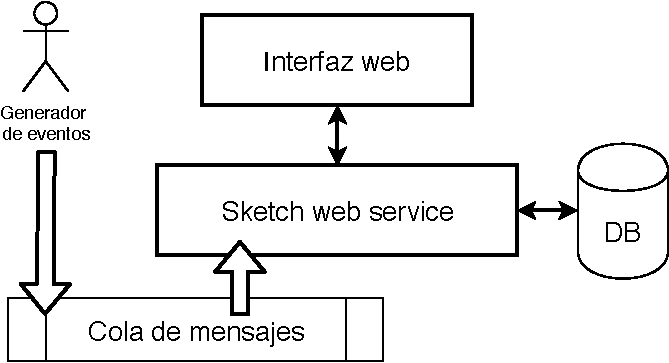
\includegraphics[width=.6\textwidth]{./graph/system_components_overview.pdf}
	\caption{Componentes del sistema}
	\label{fig:system_components_overview}
	\medskip
	\small
\end{figure}

La interfaz web consume los recursos REST expuestos por el servicio principal para presentarlos de manera convenientemente. La interacción entre el servicio y el resto de los componentes se realiza usando los conectores correspondientes disponibles para el lenguaje de programación utilizado.

\subsection{Implementación del sistema}
A continuación se describirán las entidades que conforman el sistema y los mensajes que intercambian, así como sus responsabilidades. Como se mencionó anteriormente, el proceso de detección de \textit{heavy keys} involucra dos flujos:
\begin{itemize}
	\item Actualización de la estructura de datos con cada nuevo elemento que llega al sistema.
	\item Detección de elementos anómalos en las estructuras de datos. 
\end{itemize}

El segundo flujo debe ocurrir a intervalos regulares de tiempo, a los que llamamos épocas de detección. Al finalizar cada época, se deben ejecutar los algoritmos de detección descritos en la sección \ref{sec:tecnicas_elementos_frecuentes}. Como el algoritmo de detección de \textit{heavy changers} requiere dos \textit{sketches} adyacentes en el tiempo, el sistema debe mantener una historia de los objetos generados para ejecutar este algoritmo. Esta lógica de manejo de \textit{sketches} está contenida en la entidad \textit{SketchManager}.

En la figura \ref{fig:system_components} se detallan las entidades del servicio y sus relaciones.
 
\begin{figure}[h]
	\centering
	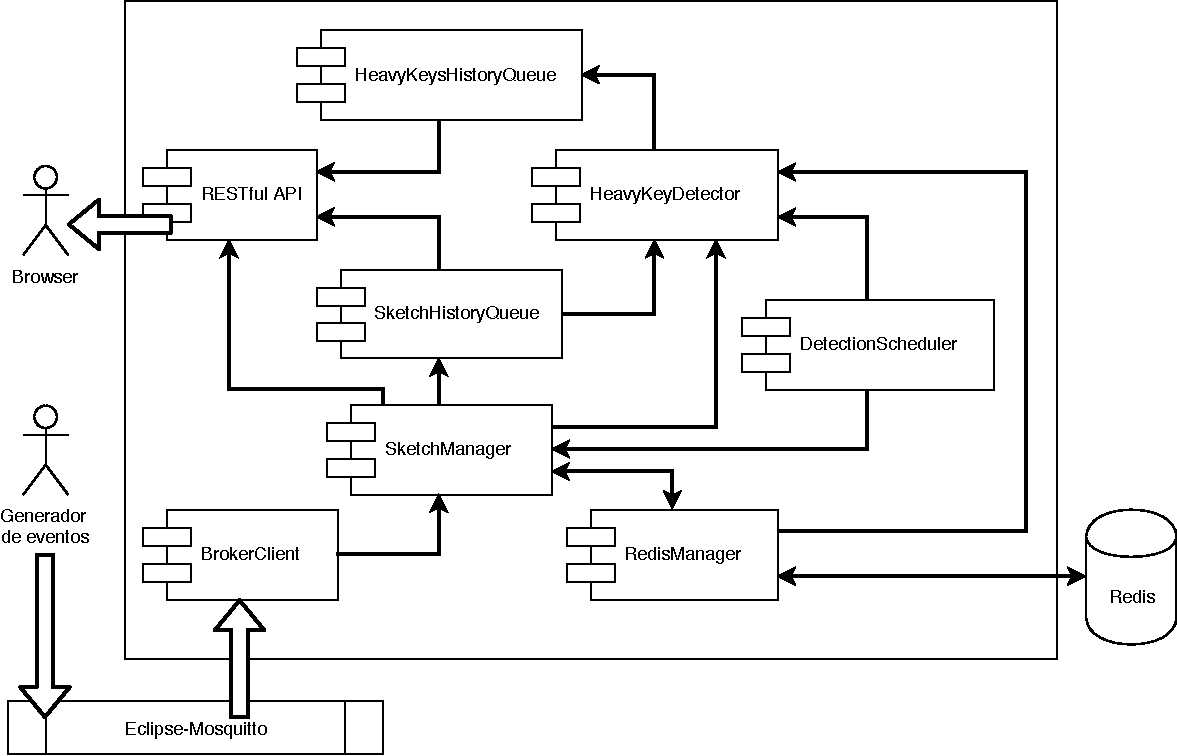
\includegraphics[width=0.9\textwidth]{./graph/system_components.pdf}
	\caption{Entidades del sistema y su interacción}
	\label{fig:system_components}
\end{figure}

Cada vez que un nuevo evento es publicado en la cola de mensajes, la entidad \textit{BrokerClient} (encargada de abstraer la lógica de conexión y manejo de errores en la interacción con la cola de mensajes) notifica a \textit{SketchManager} enviando el evento codificado como una cadena de caracteres. El valor entero asociado al evento se obtiene mediante \textit{RedisManager}, cuya responsabilidad es la de asignar un nuevo valor o retornar uno previamente asignado. La figura \ref{diag:redis_manager} se muestra el diagrama de secuencia de la entidad.

\begin{figure}[hb]
	\centering
	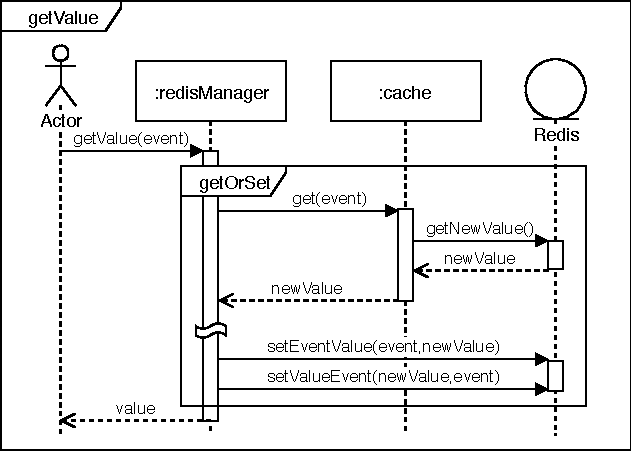
\includegraphics[width=0.6\textwidth]{./graph/SecDiag-redisManagerGetValue.pdf}
	\caption{Diagrama de secuencia asociación de valor entero a evento.}
	\label{diag:redis_manager}
\end{figure}

Para determinar el valor que será asociado al evento, \textit{RedisManager} utiliza una base de datos clave-valor donde persistir las asociaciones. Para reducir la carga, se utiliza una cache intermedia cuyo tamaño puede ser configurado a la hora de iniciar el servicio. De esta forma, cuando se consulta por el elemento a la cache, esta retorna el valor inmediatamente (si fue consultado previamente) o realiza la consulta a la base de datos y mantiene localmente el resultado de dicha consulta. 

La segunda parte del flujo ocurre solo cuando un evento sucede por primera vez, es decir, no existe en la base de datos. Como el proceso de detección utiliza números enteros, una vez que se obtiene el conjunto de \textit{heavy keys} es necesario transformar los números enteros a las cadenas de caracteres correspondientes. Para hacer esta transformación de manera eficiente, se almacenan dos asociaciones en la base de datos:
\begin{itemize}
	\item Una directa: $string \rightarrow entero$.
	\item Una inversa: $entero \rightarrow string$.
\end{itemize}

Si bien esto tiene un costo adicional en términos de espacio, permite realizar los \textit{reverse lookup} de manera directa, evitando tener que recorrer la lista de asociaciones $string \rightarrow entero$ hasta encontrar el entero buscado. Además, el motor de base de datos utilizado permite obtener un conjunto de asociaciones en una única consulta, lo cual evita establecer una conexión por cada \textit{heavy key} identificado.

La figura \ref{diag:add_event} muestra la interacción entre las tres entidades descritas anteriormente.

\begin{figure}[h]
	\centering
	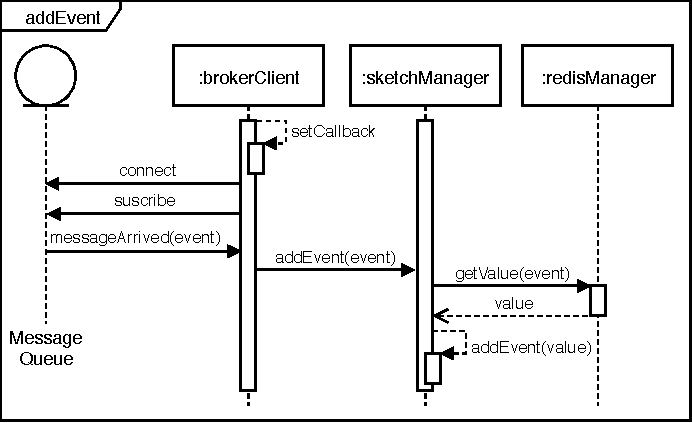
\includegraphics[width=0.7\textwidth]{./graph/SecDiag-resourceAddEventMosquitto.pdf}
	\caption{Diagrama de secuencia nuevo evento.}
	\label{diag:add_event}
\end{figure}

\

Los procesos que deben ocurrir a intervalos de tiempo regulares para la detección de \textit{hevy keys} son orquestados por la entidad \textit{DetectionScheduler} (ver figura \ref{fig:system_components}). Al final de cada época se invocan dos procesos: 
\begin{itemize}
	\item El primero provoca la generación de un nuevo \textit{sketch} que reemplaza al activo. Este último se almacena en una cola, que es manejada por la entidad \textit{SketchHistoryQueue}.
	\item El segundo proceso encapsula toda la lógica de detección de \textit{heavy keys} en la entidad \textit{HeavyKeyDetector}.
\end{itemize}

Dado que estos procesos son centrales es necesario detallar su funcionamiento y resaltar algunos puntos relacionados a implementación.
La figura \ref{diag:sketch_rotation} muestra el diagrama de secuencia de la rotación de un \textit{sketch}. Para mantener un \textit{sketch} activo e implementar el método de rotación se utilizó una cache de un único elemento. Cada vez que \textit{DetectionScheduler} envía la señal de fin de época a \textit{SketchManager} el elemento de la cache es invalidado, provocando su remoción. La cache está configurada para que cada vez que un elemento es invalidado, se ejecute un \textit{callback} que provoca la inserción del objeto en \textit{SketchHistoryQueue}.
Cuando un elemento o evento es añadido usando el método correspondiente en \textit{SketchManager} (ver figura \ref{diag:add_event}), primero se intenta recuperar el \textit{sketch} disponible en la cache. Si este existe es devuelto inmediatamente; de lo contrario, es decir, si todavía no se generó ningún objeto o si fue invalidado recientemente, la cache invoca la generación de un nuevo objeto \textit{sketch}, el cual será utilizado por todo lo que dure la época de detección. 

\begin{figure}[h]
	\centering
	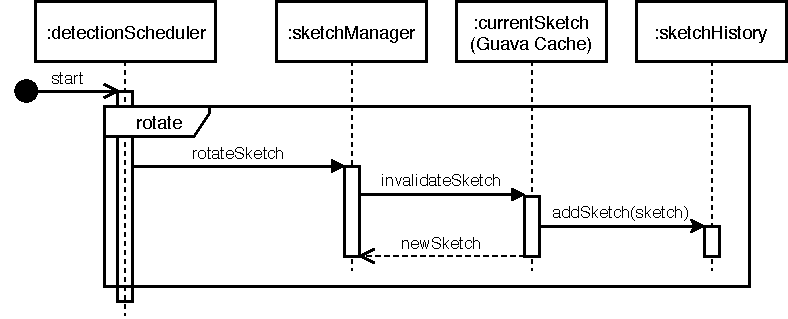
\includegraphics[width=0.7\textwidth]{./graph/SecDiag-detectionSchedulerRotation.pdf}
	\caption{Diagrama de secuencia rotación de sketches.}
	\label{diag:sketch_rotation}
\end{figure}

Luego de la rotación del \textit{sketch} se invoca el proceso de detección de \textit{heavy keys}. En la figura \ref{diag:hk_detection} puede observarse el diagrama de secuencia correspondiente. Una vez \textit{DetectionScheduler} da por finalizada una época, \textit{HeavyKeyDetector} recupera los dos \textit{sketches} más recientes que estén disponibles. Si bien es necesario solo un \textit{sketch} para realizar la detección de \textit{heavy hitters}, los \textit{heavy changers} solo pueden ser determinados entre épocas por lo que es necesario contar con los objetos de épocas adyacentes. Una vez se ejecutan los algoritmos de detección desarrollados en la sección \ref{sec:tecnicas_elementos_frecuentes} se obtiene un conjunto de números enteros, los cuales están asociados a cadenas de caracteres que representan los eventos (puntualmente el segmente TCP/IP). Para más información de la representación interna de los datos, ver la sección \ref{sec:modelado_del_problema}. Una vez obtenidos las cadenas de caracteres que identifican a aquellos elementos identificados como \textit{heavy keys}, estos se agregan a un histórico que es representado por \textit{HeavyKeysHistoryQueue}.

\begin{figure}[h]
\centering
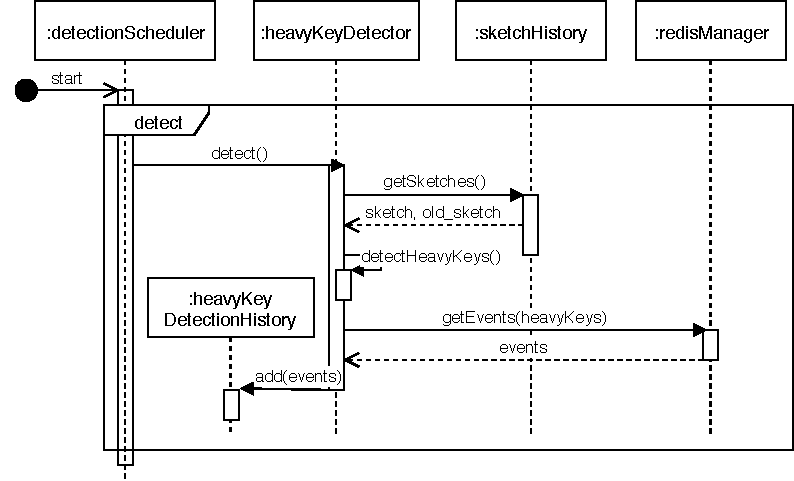
\includegraphics[width=0.7\textwidth]{./graph/SecDiag-detectionSchedulerDetect.pdf}
\caption{Diagrama de secuencia detección de \textit{heavy keys}.}
\label{diag:hk_detection}
\end{figure}

Finalmente, la API REST pone a disposición los recursos necesarios para acceder a la información que es determinada por los flujos desarrollados. Así, la interfaz web o \textit{frontend} del sistema pueden mostrar esta información de manera conveniente. Además, cualquier otra aplicación desarrollada por terceros podría consumir esta información para generación de alarmas o para disparar otros procesos.

\subsection{Recursos REST}
Los recursos expuestos por el servicio se acceden mediante las siguientes URIs.

\begin{itemize}
	\item GET     /health
	\item GET     /heavykeys
	\begin{itemize}
		\item Parámetros: count (tipo: string)
	\end{itemize}
	\item GET     /heavykeys/heavyhitters
	\begin{itemize}
		\item Parámetros: epoch (tipo: string)
	\end{itemize}
	\item GET     /heavykeys/heavychangers
	\begin{itemize}
		\item Parámetros: epoch (tipo: string)
	\end{itemize}
	\item GET     /sketchhistory
	\begin{itemize}
		\item Parámetros: count (tipo: string)
	\end{itemize}
	\item GET     /status
\end{itemize}

\subsection{Interfaz gráfica}

Una vez que los datos procesados por el sistema son presentados en forma estructurada mediante la REST API descrita anteriormente, solo resta diseñar una interfaz adecuada que muestre los datos de manera conveniente al usuario. Para esto se optó por un diseño web \textit{responsive}, con dos histogramas para presentar la ocurrencia de \textit{heavy keys} a lo largo del tiempo. Como la visualización de los datos pretende ser simple y concisa, se implementó una aplicación web de página única o SPA por sus siglas en inglés: \textit{Single-page Application}.

Además, se pueden obtener las cadenas de caracteres asociadas a cada una de ellas, por cada época, en un panel tipo lista junto a los histogramas. Finalmente, en la cabecera de la interfaz puede visualizarse el resto de la información relevante, como la cantidad total de eventos procesados y la cantidad de \textit{heavy keys} detectados (discriminados en los dos tipos desarrollados), así como la época de detección actual.

\begin{figure}[h]
	\centering
	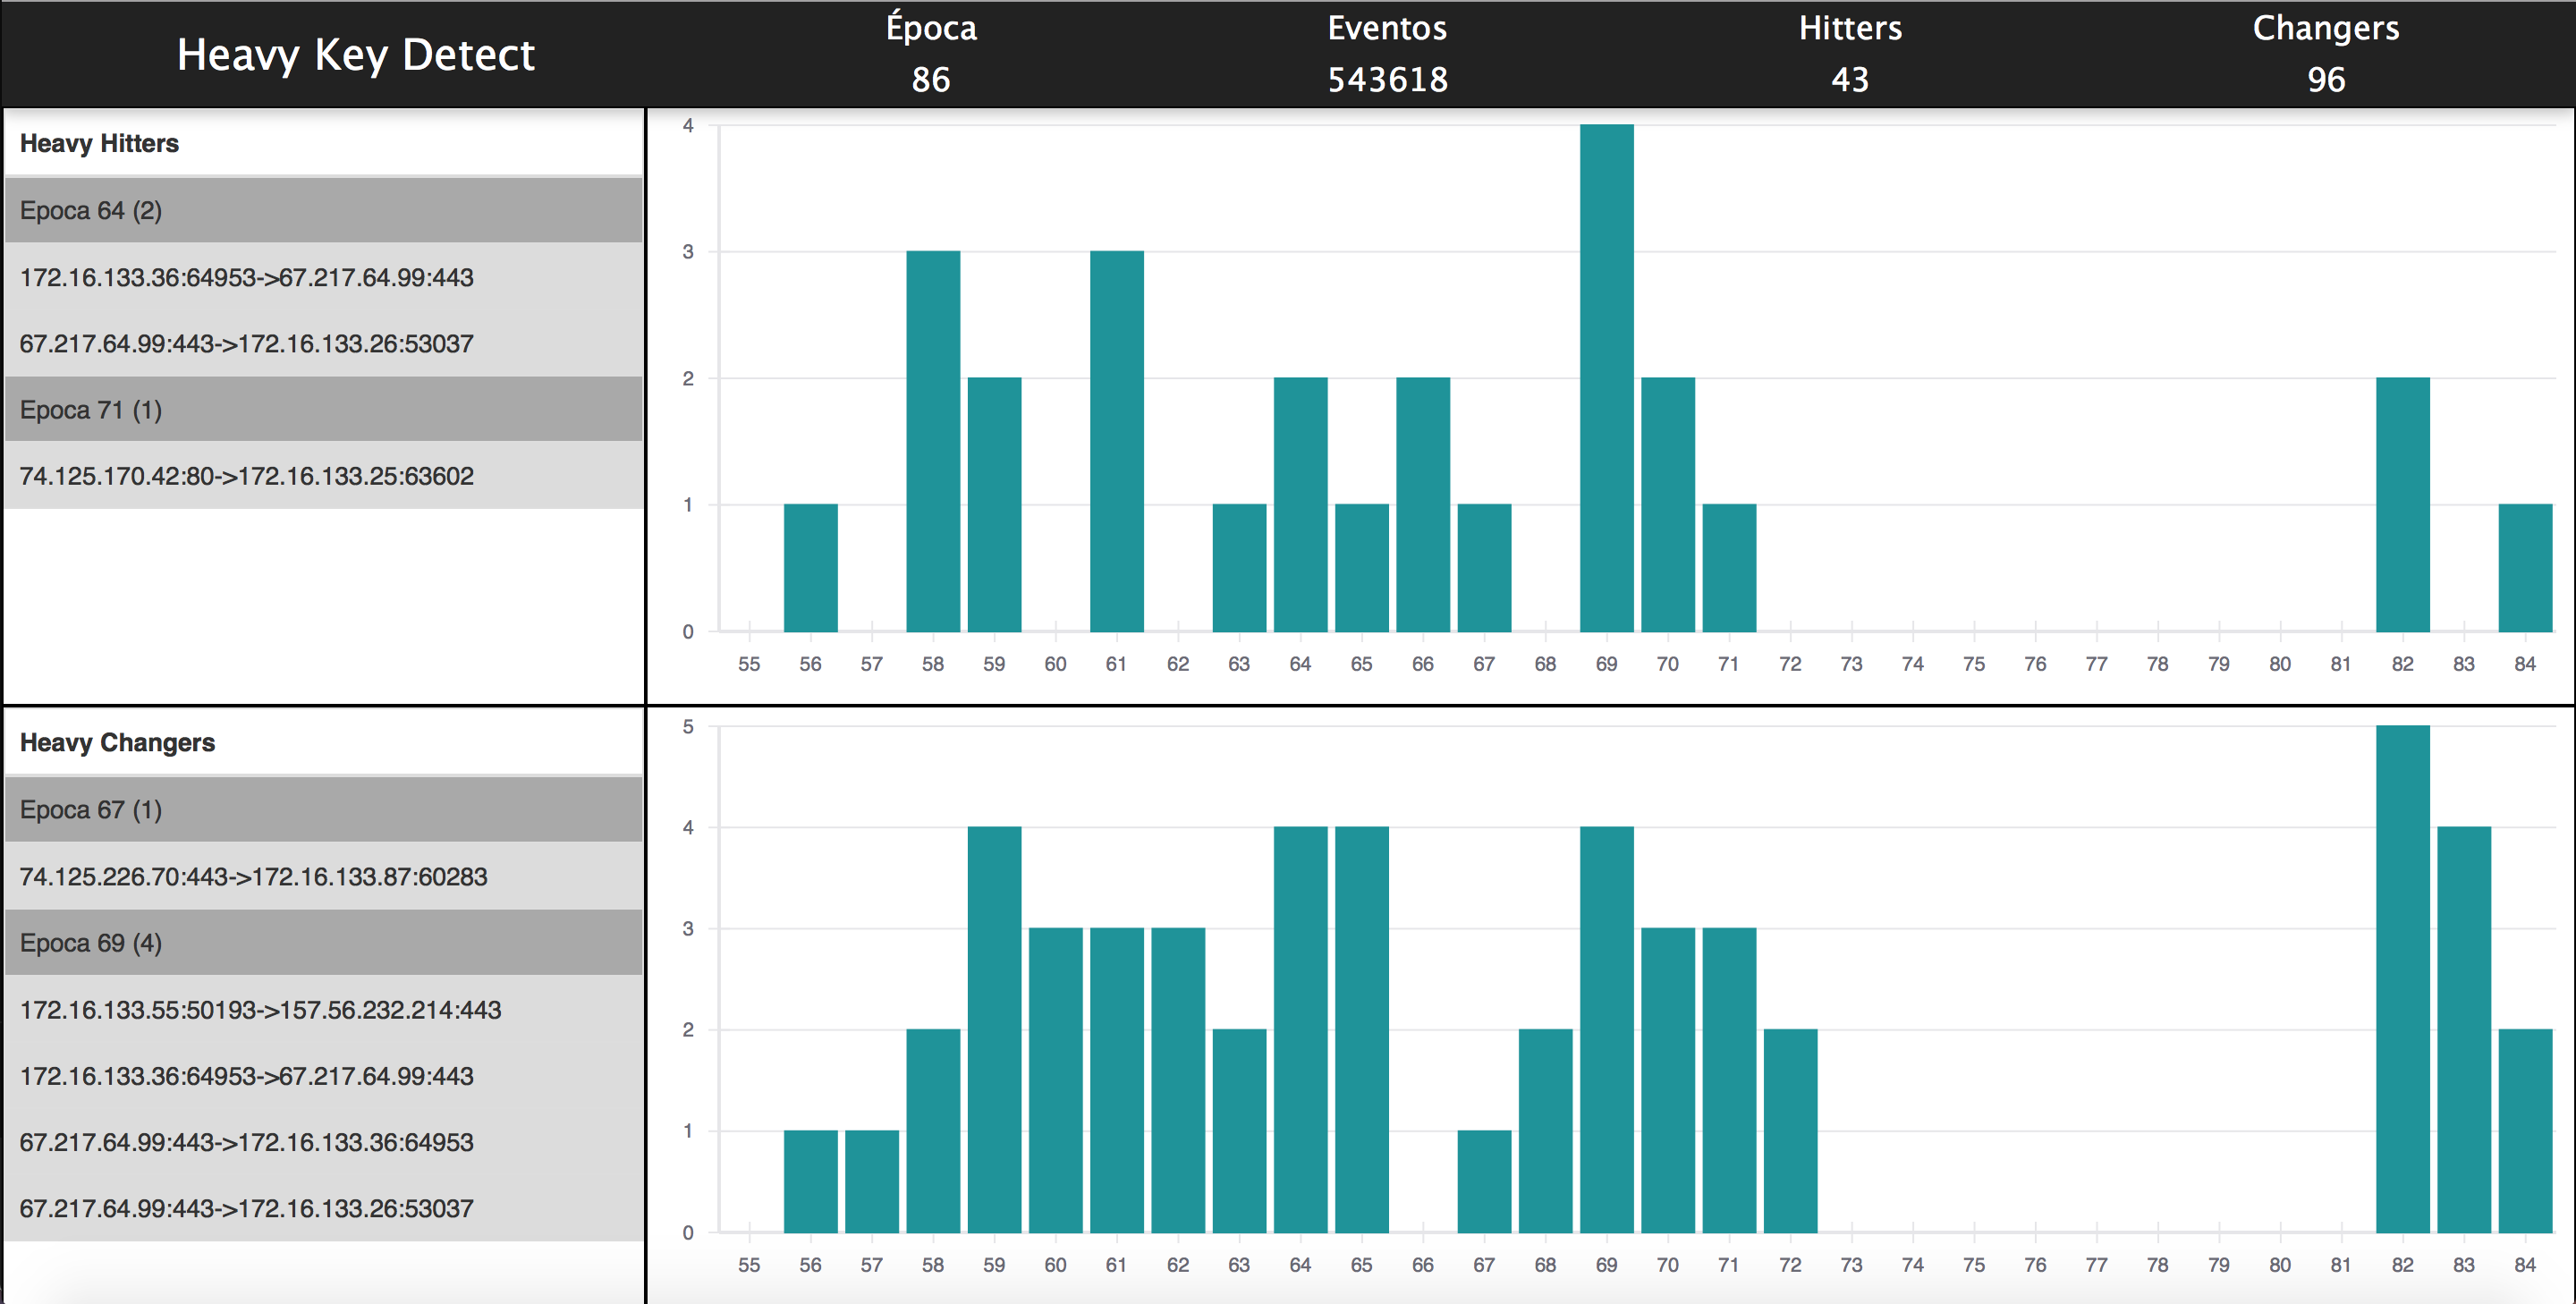
\includegraphics[width=1\textwidth]{./graph/ui.png}
	\caption{Interfaz web del sistema.}
	\label{diag:ui}
\end{figure}

Respecto a las tecnologías disponibles, existen dos estándares:
\begin{itemize}
	\item AngularJS: es un framework desarrollado y mantenido por Google Inc. Está escrito en JavaScript y hace uso del patrón de diseño MVC.
	\item ReactJS: es una librería para construir interfaces de usuario. Desarrollada y mantenida por Facebook, está pensada para diseñar vistas simples para cada estado de una aplicación. La librería es la encargada de actualizar y re-dibujar los componentes que sean necesarios cuando los datos cambian.
\end{itemize}

Si bien ambas tecnologías son ampliamente usadas y su desarrollo es sumamente activo, ReactJS parece ser la opción más conveniente dado que sus características se ajustan al problema que se intenta resolver, es decir, mostrar los datos provistos por el \textit{web-service} de manera dinámica, mientras que AngularJS ofrece un framework MVC completo que agregaría complejidad al desarollo.

En cuanto a cómo mostrar los datos, la primera aproximación consistió en el uso de una tabla con 5 columnas para fecha de detección, cantidad de \textit{Heavy Hitters}, los \textit{Heavy Hitters} detectados, cantidad de \textit{Heavy Changers} y los \textit{Heavy Changers} detectados. Sin embargo, cómo la cantidad de eventos detectados por fila es variable, hubiese sido necesario mostrar más de una dato por celda, por lo que la utilización de una tabla parecería no ser la adecuada (se asume que cada celda es atómica, es decir, debe mostrar un único dato).

Otra alternativa mas conveniente dada la naturaleza temporal de los datos, y la cantidad de ocurrencia de eventos, es utilizar un histograma con desplazamiento. Con cada desplazamiento, los datos para la nueva época son agregados. Así, puede observarse cuando ocurren ciertos eventos, y compararlos a simple vista con otros intervalos de tiempo pasados y futuros. En la imagen \ref{diag:ui} puede observase una primera implementación de la interfaz web.


\newpage

\section{Telemetría}
Cuando los servicios son llevados a ambientes de producción, es esencial poder monitorear diferentes métricas de manera remota. Más aún, es importante llevar un registro de la historia de dichas métricas para entender cómo se comporta el sistema a lo largo del tiempo, tanto cuando es sometido a diferentes cargas como cuando se presenta algún problema que interrumpe su funcionamiento o degrada sus rendimiento. Además, cuando se implementa adecuadamente, la telemetría puede ser usada para entender en tiempo real como los usuarios hacen uso de la aplicación.

Telemetría se define como un proceso automático de comunicación por el que mediciones y otros datos son recolectados y transmitidos a los equipos con los que se realizan tareas de monitoreo. En el mundo de las aplicaciones en la nube, se debe controlar la salud y la performance de las aplicaciones constantemente, de manera remota. Los datos de telemetría provienen de logs, métricas y eventos. Usualmente, las mediciones se relacionan al consumo de memoria, uso de CPU y tiempos de respuesta de bases de datos, entre otros.

Los casos de uso principales para monitorear eventos, logs y métricas pueden catalogarse en las siguientes categorías:
\begin{itemize}
	\item Tiempo fuera de servicio: consiste en controlar la ocurrencia de inconvenientes en los sistemas en producción para resolverlos lo más rápido posible.
	\item Monitoreo del producto: analizar y comprender el comportamiento de los usuarios para mejorar el producto o servicio que se está prestando.
	\item Predecir anomalías futuras: anticiparse a los problemas antes de que ocurran.
	\item Seguridad: controlar proactivamente la existencia de fallas de seguridad
\end{itemize}

Para implementar una solución de telemetría de utilidad, es necesario decidir que datos son importantes y determinar que logs, eventos y métricas se relacionan con los KPI (\textit{Indicadores Clave de Performance}). Además de los datos de la aplicación en sí, también es importante monitorear constantemente la infraestructura que hace posible que el servicio funcione. Para este desarrollo, es necesario desplegar un conjunto de servicios para almacenar y comunicar los datos de telemetría del servicio encargado de hacer la detección de anomalías. El gráfico muestra los servicios desplegados y su interacción\footnote{Si bien el sistema está diseñado para ser desplegado en un cluster de servidores, los servicios se ejecutan en un único equipo haciendo uso de tecnologías de virtualización.}:

\begin{figure}[h]
	\centering
	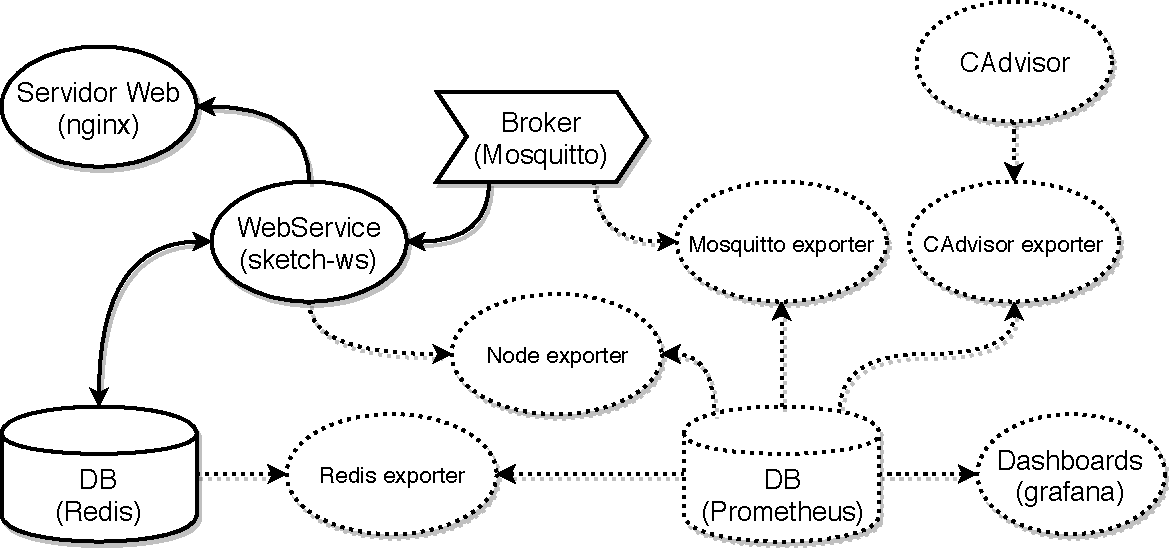
\includegraphics[width=0.9\textwidth]{./graph/service_infrastructure.pdf}
	\caption{Infraestructura completa del servicio, incluyendo telemetría.}
	\label{diag:service_infrastructure}
\end{figure}

Los servicios y flujos que están dibujados con lineas completas fueron los que se mostraron en la figura \ref{fig:system_components}. Aquellos en lineas punteadas son los utilizados para implementar telemetría en todos los componentes. Cada uno de los 'exporter' es el encargado de recolectar la información que publican los servicios y escribirla en una base de datos de series de tiempo. Luego, con la información temporal disponible, es posible agregar dicha información y mostrarla en forma organizada.

Además de los parámetros básicos de uso de CPU, memoria y utilización de recursos de red de cada una de las instancias del sistema, el servicio principal fue instrumentado para exponer una serie de métricas de interés:

\begin{itemize}
	\item Cantidad de eventos procesados por segundo.
	\item Cantidad de \textit{heavy keys} detectadas por época.
	\item Cantidad de clientes conectados, publicando eventos.
	\item Cantidad de mensajes recibidos (Broker).
	\item Uso de memoria y cantidad de hilos de la JVM.
\end{itemize}

En base a la información agregada se pueden construir \textit{dashboards} que resumen el comportamiento del sistema a lo largo del tiempo, y el estado del mismo. Estas pantallas resultan de suma utilidad para quien esté monitoreando el servicio, dado que permiten visualizar el estado general de toda la infraestructura. En los anexos se incluyen capturas de pantalla de las dos vistas más relevantes con respecto a telemetría.

La base de datos utilizada tiene una característica particular con respecto a las bases de datos convencionales de series de tiempo. Cómo se desarrollará más adelante, el mecanismo por el cual se obtienen los datos es una característica diferenciadora, lo cual se evidencia en la dirección de las flechas que salen de la base de datos a los componentes: aunque parece contraintuitivo, delegar la responsabilidad de obtener los datos a la base de datos evita problemas de sincronismo y evita instrumentación necesaria en el código del componente.

\newpage

\section{Tecnologías utilizadas}\label{sec:tecnologias_utilizadas}

Dados los distintos tipos de desafíos que se fueron presentando en el desarrollo del proyecto, fue necesario implementar soluciones a los mismos haciendo uso de alguna de las tecnologías disponibles actualmente. En muchos casos es posible encontrarse con que varios tipos de tecnologías resuelven problemas similares, pero que cada una tiene una característica particular que la diferencia y la hace más o menos aplicable a ciertas situaciones.

\subsection{Desarrollo del servicio principal}
Con respecto a la selección del lenguaje de programación, Java\cite{java} es prácticamente la única opción disponible cuando se quiere construir sistemas de alto desempeño y robustez. Es un lenguaje maduro, ampliamente adoptado por compañias alrededor del mundo y dispone de librerías para la gran mayoría de las tecnologías existentes. El sistema utiliza \textit{OpenJDK} en su versión 8, dado que introduce, entre muchas características, el uso de expresiones lambda. Estas permiten explotar las capacidad de cómputo paralelo de los sistemas con múltiples núcleos, lo cual es esencial para las aplicaciones de \textit{data streaming}.

Respecto a la elección del \textit{framework} de desarrollo, se optó por \textit{Dropwizard}\cite{dropwizard}. El mismo permite construir \textit{RESTful webservices} de alta performance brindando soporte nativo para manejo de configuraciones y métricas de aplicación. Además, brinda la posibilidad de empaquetar todas las dependencias en un único artefacto, evitando la necesidad de configurar y mantener servidores HTTP para ejecutar el código de la aplicación. Utiliza \textit{Jetty}\cite{jetty} para HTTP, haciendo posible embeber el servidor web junto con el código, \textit{Jersey}\cite{jersey} para construir aplicaciones web RESTful, \textit{Jackson}\cite{jackson} para dar formato a los objetos JSON y \textit{Metrics}\cite{metrics} para generar métricas del servicio.

Una librería adicional utilizada es \textit{Guava}\cite{guava}. Es un conjunto de librerías \textit{core} mantenido por Google, que incluye nuevos tipos de colecciones cómo \textit{multimaps} y \textit{multisets}, colecciones inmutables, una librería de grafos y implementaciones de caches de distintos tipos, por nombrar algunas de las tantas características que tiene.

\

El desarrollo y despliegue del servicio se basan en la plataforma de contenedores \textit{Docker}\cite{docker}. Permite empaquetar aplicaciones y sus dependencias en contenedores virtuales que pueden ejecutarse en cualquier sistema operativo. Puede integrarse con varias herramientas de infraestructura como AWS, Ansible, Google Cloud Platform, Kubernetes, Puppet, Vagrant, entre otros.
Además, permite construir flujos de integración continua dado que cada nueva versión de código puede ser empaquetada en cuestión de minutos e integrada con el resto de la infraestructura con solo cambiar el contenedor correspondiente. Mediante el uso de repositorios centrales como \textit{DockerHub}, brinda la posibilidad de construir y distribuir automáticamente nuevos paquetes de código.
Finalmente, el uso de \textit{docker-compose} permite definir y ejecutar aplicaciones multi-contenedor, usando un archivo YAML para configurar los servicios de la aplicación y una interfaz de linea de comandos para orquestar la creación y ejecución de todos los contenedores. La infraestructura definida en la figura \ref{diag:service_infrastructure} está codificada en el archivo \textit{docker-compose.yml}, disponible en el repositorio del servicio\cite{sketch-service}. Allí pueden encontrarse también las instrucciones para desplegar todos los componentes en cualquier sistema operativo GNU/Linux con ambas herramientas instaladas.


\subsection{Base de datos clave-valor}
Como se discutió en la sección \ref{sec:modelado_del_problema}, la necesidad de asociar valores con cadenas de caracteres en un repositorio centralizado que pueda ser accedido de manera eficiente hace necesaria la utilización de una base de datos clave-valor.
Este tipo de base de datos surge como una alternativa a las limitaciones de las base de datos relacionales (RDB), donde los datos son estructurados en tablas cuyo esquema debe ser predefinido. En las bases de datos \textit{NoSQL}, no existe esquema y el valor del dato es opaco. Los valores son identificados y accedidos mediante una clave, y los valores almacenados pueden ser números, strings, contadores, JSON, XML, HTML, binarios, imágenes, entre otros. Es el modelo \textit{NoSQL} más flexible porque la aplicación tiene control absoluto sobre lo que es almacenado como valor.

Muchas aplicaciones que no se adaptan al modelo tradicional RDB pueden beneficiarse del modelo \textit{clave-valor}, dado que ofrece una serie de ventajas:

\begin{itemize}
	\item Modelado de datos flexible: dado que los datos no deben tener una estructura compatible con un esquema, estas bases de datos ofrecen mucha flexibilidad para modelar los datos de forma que cumplan los requerimientos de la aplicación.
	\item Alta performance: la arquitectura \textit{clave-valor} puede ser mucho más eficiente que la RDB en muchos escenarios dado que no existe la necesidad de utilizar locks, join, union u otras operaciones cuando se trabaja con objetos. A diferencia de las RDB, un almacén \textit{clave-valor} no necesita realizar búsquedas entre columnas o tablas para encontrar un objeto: dada la clave es posible obtener la ubicación del objeto rápidamente.
	\item Simplicidad operacional: algunas bases de datos están diseñadas específicamente para simplificar su operación, facilitando los mecanismos para agregar o quitar capacidad si es necesario, y asegurando que fallas en hardware o redes no generen tiempos fuera de servicio.
\end{itemize}

Dados los requerimientos de alto desempeño no es posible persistir los datos en disco. Por este motivo, es necesario optar por una base de datos en memoria. Entre las más conocidas, se evaluaron dos alternativas:

\begin{itemize}
	\item Memcached: es un sistema distribuido para cacheo de memoria. Se utiliza para almacenar objetos en memoria de forma de reducir el número de veces que se consultan fuentes de datos externas. Básicamente, Memcached es una gran tabla de hash distribuida en muchos equipos.
	\item Redis: es una base de datos \textit{clave-valor} en memoria, con la opción de persistencia. Maneja distintos tipos de estructuras de datos abstractas como strings, listas, conjuntos, etc.
\end{itemize}

Si bien Memcached es superior en performance, Redis brinda la posibilidad de persistir los datos en disco. Esto puede resultar ventajoso si se pretende pausar el servicio o si una eventual falla implica reiniciar el servicio: guardando estados de la base de datos a intervalos regulares de tiempo permite seguir trabajando con una pérdida muy pequeña de información, o si el servicio es pausado, permite reanudar su funcionamiento de manera inmediata.

\subsection{Telemetría}
Para analizar los datos de telemetría de forma adecuada, es necesario persistirlos en un soporte adecuado. En la actualidad, existen diferentes tipos de bases de datos de series de tiempo, cada una con sus características diferenciadoras. Para este proyecto se optó por \textit{Prometheus}.
\

\textit{Prometheus} es más que una bases de datos de series de tiempo, es un sistema completo de monitoreo y alerta. La característica diferenciadora que hace tan popular a esta tecnología es la forma en que los datos se escriben en la base de datos. En los anexos puede verse un diagrama de su arquitectura. Los datos almacenados en \textit{Prometheus Server} (que es la base de datos en sí) son persistidos mediante un mecanismo de \textit{pulling}: una serie de \textit{exporters} exponen las distintas métricas mediante una interfaz \textit{REST} que es consumida por el servidor y almacenada en la base de datos. Los \textit{exporters} permiten integrar los distintos servicios de manera transparente, y proveen una interfaz que evita acoplar lo componentes con la solución de telemetría. Estos pueden observarse en la figura \ref{diag:service_infrastructure}.

\subsection{Monitoreo de los contenedores}
\textit{cAdvisor} es un demonio que colecta, agrega, procesa y exporta información acerca de los contenedores que están ejecutándose en el sistema. Permite entender el uso de recursos y las características de performance de los mismos. Es mantenido por Google y es el estandar para monitoreo de contenedores.


\newpage

\section{Pruebas realizadas}
Se realizaron dos experimentos para comprobar el funcionamiento del servicio. En el primero se generaron una serie de eventos en el tiempo con un patrón en particular. En el segundo experimento se utilizaron los flujos TCP/IP de una captura de tráfico de red para generar los eventos generados por un equipo de red. 

\subsection{Patrones de eventos generados localmente}
Para el primer experimento se generaron una serie de eventos consecutivos en el tiempo, representados como un par \textit{(tiempo, evento)}. Para cada etiqueta, los eventos son espaciados regularmente en el intervalo de tiempo en el que se generaron, y se agregan pequeñas perturbaciones para evitar que la cantidad de eventos en ventanas adyacentes sea idéntica. Además, se agregan una serie de eventos aleatorios para simular situaciones reales donde pueden existir otras etiquetas que introducen ruido a la señal.

En la figura \ref{fig:prueba1} se observa la distribución de los eventos generados a lo largo del tiempo, para un intervalo de 60 segundos. Cada barra del gráfico representa un intervalo de tiempo de $3$ segundos.
Los eventos se generan para los intervalos de tiempo definidos de la siguiente manera: en el intervalo $(0,10)$ se generan $1200$ eventos $E1$, en $(10,40)$ se generan $800$ eventos $E2$, en $(33,36)$ se generan $400$ eventos $E3$, en $(40,47)$ se generan $500$ eventos $E4$ y en $(54,58)$ se generan $400$ eventos $E5$. Finalmente se suman $1500$ eventos aleatorios a toda la duración de la simulación. 

\begin{figure}[ht]
	\centering
	\makebox[0pt][c]{%
		\begin{minipage}{0.75\textwidth}
			\centering
			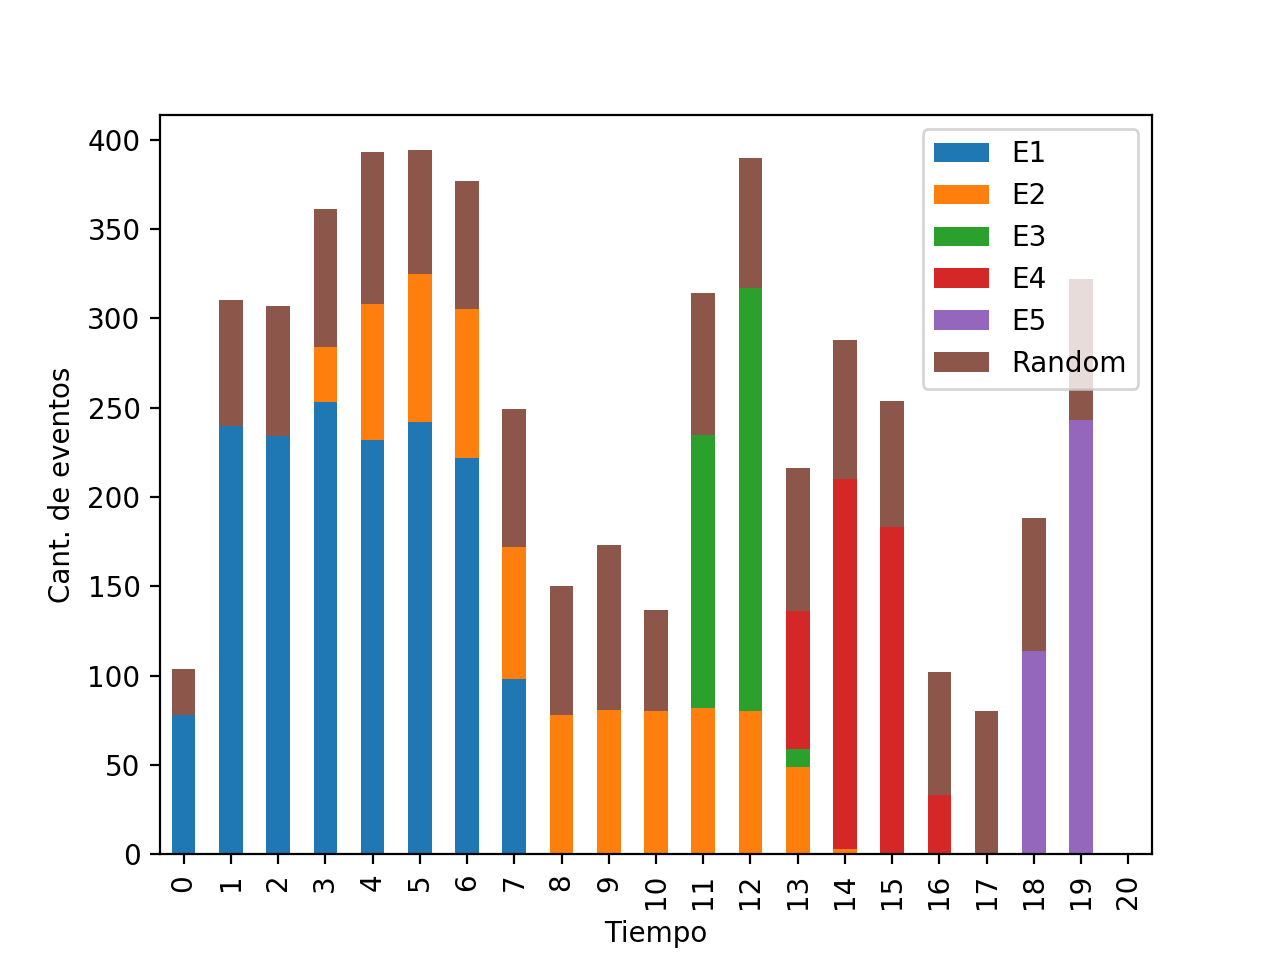
\includegraphics[scale=0.7]{graph/prueba1.png}
			\caption{Distribución de los eventos en el tiempo}
			\label{fig:prueba1}
		\end{minipage}
		\begin{minipage}{0.6\textwidth}
			\small
			\centering
			\begin{tabular}{ | l | c | c | c | c | c | c | c | c |}			
				\hline			
				Tiempo & 0 & 1 & 2 & 3 & 4 & 5 & 6 \\
				\hline
				Heavy Hitters & - & E1 & E1 & E1 & E1 & E1 & E1\\
				Heavy Changers & E1 & - & - & - & - & - & - \\
				\hline
				\hline
				Tiempo & 7 & 8 & 9 & 10 & 11 & 12 & 13  \\
				\hline
				Heavy Hitters & E1 & - & - & - & - & E3 & - \\
				Heavy Changers & E1 & - & - & - & E3 & E3 & E3 \\
				\hline\hline
				Tiempo & 14 & 15 & 16 & 17 & 18 & 19 & 20 \\
				\hline
				Heavy Hitters & - & E4 & E4 & - & - & E5 & - \\
				Heavy Changers & E4 & - & E4 & - & E5 & E5 & - \\
				\hline
			\end{tabular}
			\caption{HeavyKeys detectadas}
			\label{tab:prueba1}
		\end{minipage}
	}%
\end{figure}

Comprobando los resultados de la detección, se puede observar un defasaje entre los eventos detectados y los mostrados en la figura \ref{fig:prueba1}. Esto es así debido a que la simulación no inicia necesariamente en el comienzo de una época de detección (es decir, al comienzo de la ventana de tiempo de $3$ segundos configurada para este experimento). Por ejemplo, $E1$ es reportado como \textit{heavy changer} al momento $0$ cuando en realidad debería pasar inadvertido. Sin embargo, en el siguiente intervalo es reportado correctamente.
De la misma manera, podemos ver que el evento $E2$ no es reportado dado que esta por debajo de los límites configurados.

\

Los parámetros con los que el servicio estaba configurado a la hora de realizar esta prueba son: 

\begin{multicols}{2}
	\begin{itemize}
		\item Sketches
		\begin{itemize}
			\item rows(5)
			\item cols(100)
			\item prime(7283)
		\end{itemize}
	\end{itemize}
	\columnbreak
	\begin{itemize}
		\item Detección
		\begin{itemize}
			\item heavyHitterThreshold(150)
			\item heavyChangerThreshold(100)
			\item sketchRotationInterval(3)
		\end{itemize}
	\end{itemize}
\end{multicols}

\subsection{Trafico de red}
En esta prueba se utilizó un archivo de captura de tráfico de red para emular el comportamiento de los paquetes que atraviesan una interfaz de red. Este dataset, que es usado en la suite \textit{Tcpreplay\footnote{http://tcpreplay.appneta.com/wiki/captures.html}} para probar performance en switches y adaptadores de red, esta diseñado para generar una gran cantidad de flujos usando varios protocoles, manteniendo bajo el tráfico promedio de la red. Contiene 15000 paquetes de red y una duración de 300 segundos.

\begin{figure}[h!]
	\centering
	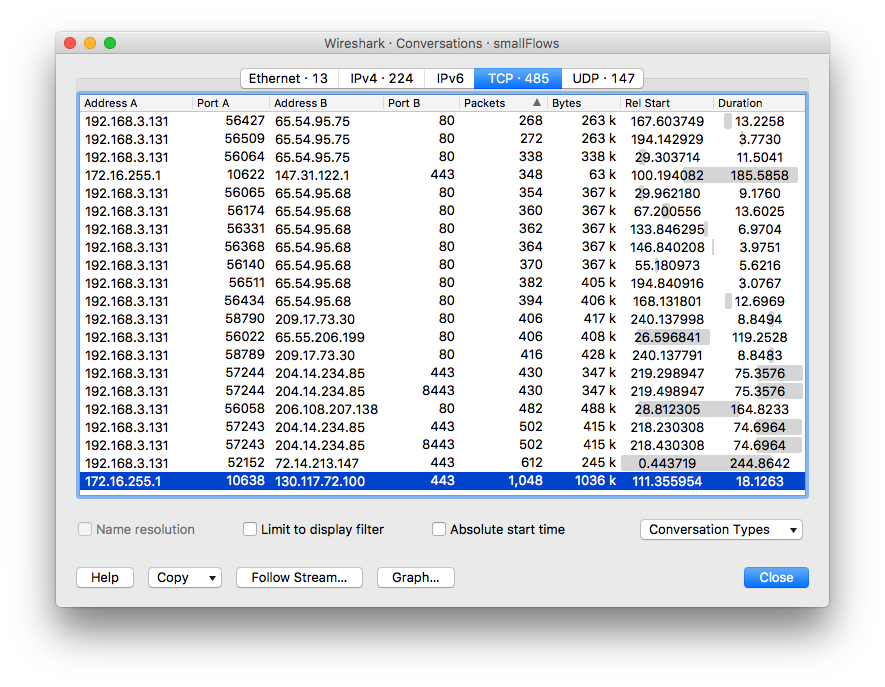
\includegraphics[width=.9\textwidth]{graph/smallFlows_conversations.png}
	\caption{Conversaciones TCP del archivo de captura de tráfico de red}
	\label{fig:smallFlows_conversation}
	
\end{figure}

Analizando los flujos que se muestran en la figura \ref{fig:smallFlows_conversation} se puede observar que la conversación con mayor cantidad de paquetes ocurre entre las direcciones 130.117.72.100:443 y 172.16.255.1:10638. A partir del instante $111.35$ se intercambian $1048$ paquetes en un período de $18.12$ segundos, que son detectados correctamente como \textit{heavy changers}. Los parámetros con los que se configuró el sistema son similares a los usados en el experimento anterior, solo que se aumentaron los umbrales: \textit{heavyHitterThreshold} es $250$ y \textit{heavyChangerThreshold} es $200$.


\subsection{Mejoras de performance}
\subsubsection{Implementación inicial: REST API}
En la implementación inicial se había optado por registrar la ocurrencia de eventos usando una interfaz REST API, mayormente por la sencillez de su implementación y el amplio soporte y adopción que tiene esta tecnología en el mundo de los \textit{webservices}. Sin embargo, se observa que cuando se intentan procesar cantidades masivas de eventos en tiempo real, el sistema evidencia una \textit{performance} pobre dada la naturaleza síncrona de la comunicación.

Los resultados de las pruebas que serán mostradas a continuación, se realizaron en un sistema con las siguientes característica: procesador AMD FX6300 a $2.5$ GHz, 8GB de memoria RAM, sistema operativo \textit{Ubuntu Linux 16.04}, kernel \textit{GNU/Linux 4.13.0.32-generic}.

Para determinar el volumen real de eventos que el sistema puede manejar, se generaron datos sintéticos y se registraron en el sistema de manera consecutiva por un lapso de 10 minutos, sin espera entre la registración de cada evento. El gráfico \ref{fig:REST} muestra la cantidad de eventos procesados a lo largo del tiempo.

\begin{figure}[h]
	\centering
	\begin{tikzpicture}
	\begin{axis}[
	axis x line=middle,
	axis y line=middle,
	enlarge y limits=true,
	width=12cm, height=8cm,     % size of the image
	grid = major,
	grid style={dashed, gray!30},
	ylabel=eventos,
	xlabel=$s$,
	legend style={at={(0.1,-0.1)}, anchor=north}
	]        
	
	\addplot [no markers, red, line width=1pt] table [y={create col/linear regression={y=y}}] {data/tablerest.dat};
	\addplot[mark=diamond] table  {data/tablerest.dat};
	\end{axis}
	\end{tikzpicture}
	
	\caption{Eventos procesados a lo largo del experimento (REST API).} \label{fig:REST}
\end{figure}

La recta que mejor ajusta los datos está dada por la ecuación $y = 253.71 x + 32.1$. La pendiente de la recta sirve entonces para estimar la performance de la implementación REST del sistema en alrededor de $250$ eventos por segundo.

\subsubsection{Nueva implementación: Messaging Queue}
Para esta nueva implementación es necesario un nuevo componente en la arquitectura del sistema. Se agregó una instancia de una \textit{message queue} y se hicieron las modificaciones necesarias para que el \textit{webservice} se suscriba a un tópico determinado y procese los eventos que son allí publicados: esto implica cambiar la interfaz para la creación de nuevos eventos e implementar los callbacks necesarios.

\begin{figure}[h]
	\centering
	\begin{tikzpicture}
	\begin{axis}[
	axis x line=middle,
	axis y line=middle,
	enlarge y limits=true,
	width=12cm, height=8cm,     % size of the image
	grid = major,
	grid style={dashed, gray!30},
	ylabel=eventos,
	xlabel=$s$,
	legend style={at={(0.1,-0.1)}, anchor=north}
	]        
	
	\addplot [no markers, red, line width=1pt] table [y={create col/linear regression={y=y}}] {data/tablemq.dat};
	\addplot[mark=diamond] table  {data/tablemq.dat};
	\end{axis}
	\end{tikzpicture}
	
	\caption{Eventos procesados a lo largo del experimento (Message Queue).} \label{fig:MQ}
\end{figure}

Las pruebas realizadas son similares a las presentadas anteriormente y se realizan en el mismo sistema. Se generaron eventos aleatorios y se publicaron en un canal determinado de la cola de mensajes. Muestreando la cantidad de eventos que el sistema procesa a intervalos regulares de tiempo, se confecciono la gráfica \ref{fig:MQ}. A simple vista se puede observar un aumento pronunciado en la performance del sistema. La recta que ajusta a los datos está dada por la ecuación $y = 6907.2 x - 48449$, por lo que podemos estimar un volumen de procesamiento de alrededor de $6900$ eventos por segundo. La única desventaja de este método de envío de mensajes es que requiere que los clientes publiquen los mensajes en un canal dado, haciendo uso de las librerías correspondientes para su implementación. Además, podemos observar que la gráfica es una curva perfecta, mientras que en el caso previo se pueden observar pequeñas oscilaciones regulares a lo largo del tiempo. Esto puede deberse a procesos que JVM ejecuta en segundo plano, como el \textit{garbage collector}, dado el volumen de objetos que se crean y destruyen en memoria.

Con la implementación actual, podemos observar que la performance del sistema es 27 veces mejor que la implementación del segundo incremento. Aunque esto implica el despliegue de un servicio de cola de mensajes y escribir clientes que publiquen mensajes en la misma, la ganancia en prestaciones es lo suficientemente buena como para que el beneficio justifique los costos de desarrollo.

\subsection{Pruebas de longevidad}
Las pruebas de longevidad permiten conocer la estabilidad del sistema. Son de larga duración y permiten corroborar el comportamiento del sistema con una carga apropiada, que simula condiciones reales de uso. Usualmente, se estima cual sería una carga típica para una aplicación dada y se somete a los componentes a un múltiplo de este valor: si cierta aplicación se estima va a generar 100 eventos por segundo, entonces las pruebas de longevidad van a generar 500 eventos por segundo durante un período de varias horas. De esta manera, los desarrolladores tienen cierta confianza en que, si no ocurren fallos cuando el sistema se somete a esta prueba, tampoco ocurrirán en condiciones normales.

Luego de someter al sistema a una carga máxima constante durante 14 horas se observa que:
\begin{itemize}
	\item Se procesaron más de 10 billones de eventos en poco más de 16000 épocas.
	\item El consumo de memoria se mantiene estable durante toda la prueba.
	\item En promedio, el sistema procesó eventos a una velocidad de 20000 eventos por segundo\footnote{Las fluctuaciones que se observan en la gráfica son resultado de haber realizado las pruebas en un entorno de desarrollo}.
	\item La API de \textit{health} del sistema reporta el correcto funcionamiento de todos los componentes durante la duración de la prueba.
\end{itemize}

En las siguientes figuras pueden observarse la telemetría más relevante durante toda la prueba:
\begin{figure}[h]
	\centering
	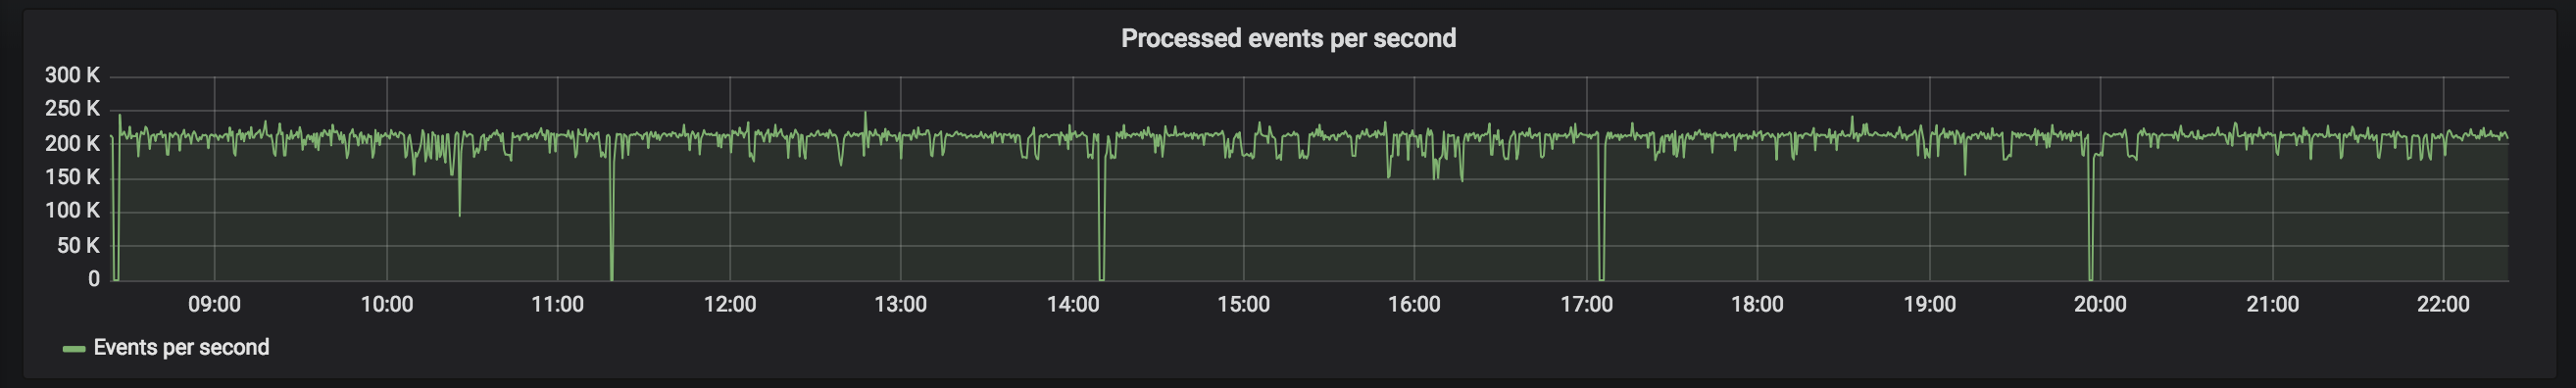
\includegraphics[width=1\textwidth]{./graph/processed_evts_per_second.png}
	\caption{Eventos procesados por segundo.}
	\label{diag:processed_evts_per_second}
\end{figure}
\begin{figure}[h]
	\centering
	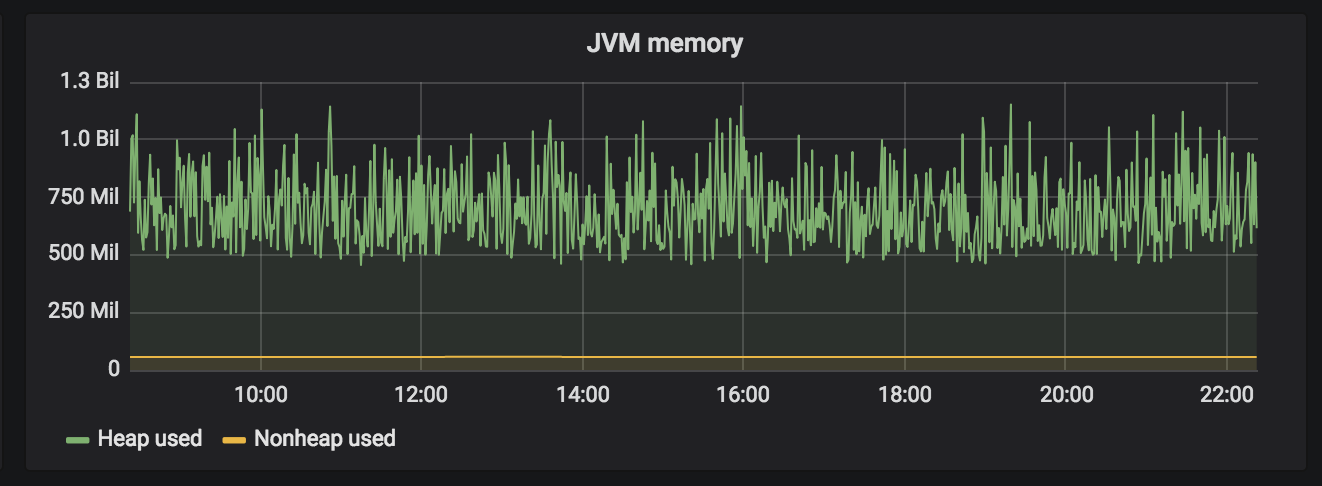
\includegraphics[width=1\textwidth]{./graph/jvm_memory.png}
	\caption{Memoria de la Java Virtual Machine.}
	\label{diag:jvm_memory}
\end{figure}
\begin{figure}[h]
	\centering
	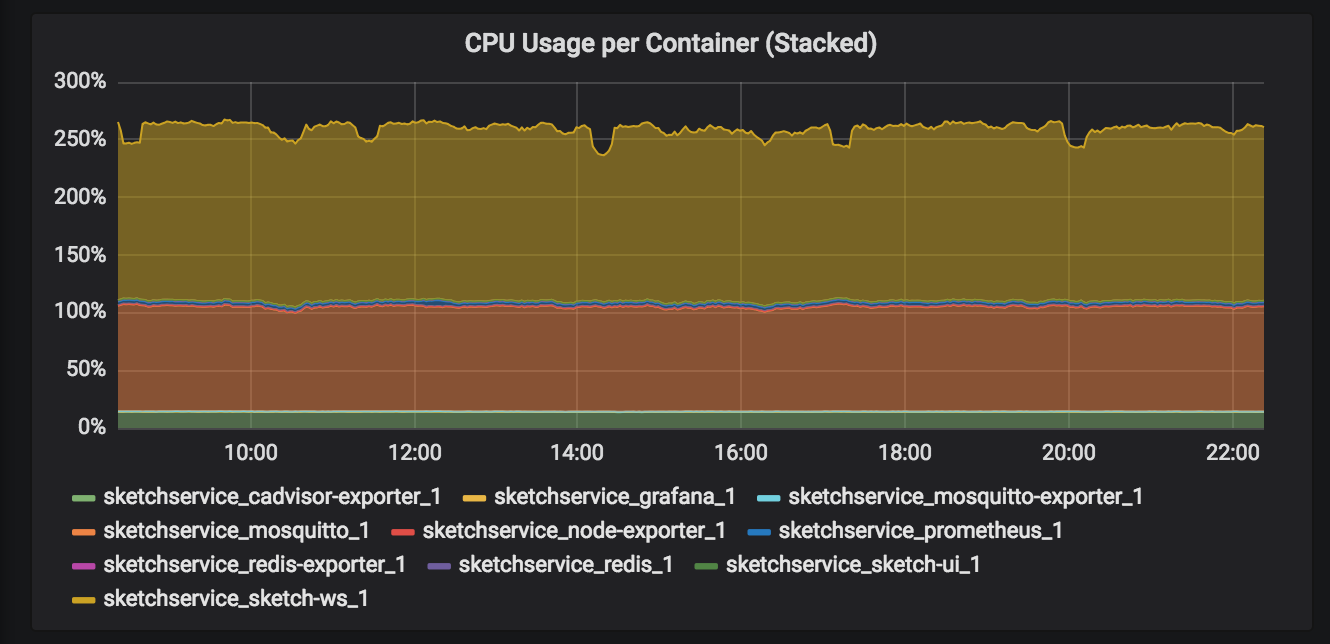
\includegraphics[width=1\textwidth]{./graph/cpu_usage.png}
	\caption{Consumo de CPU.}
	\label{diag:cpu_usage}
\end{figure}
\begin{figure}[h]
	\centering
	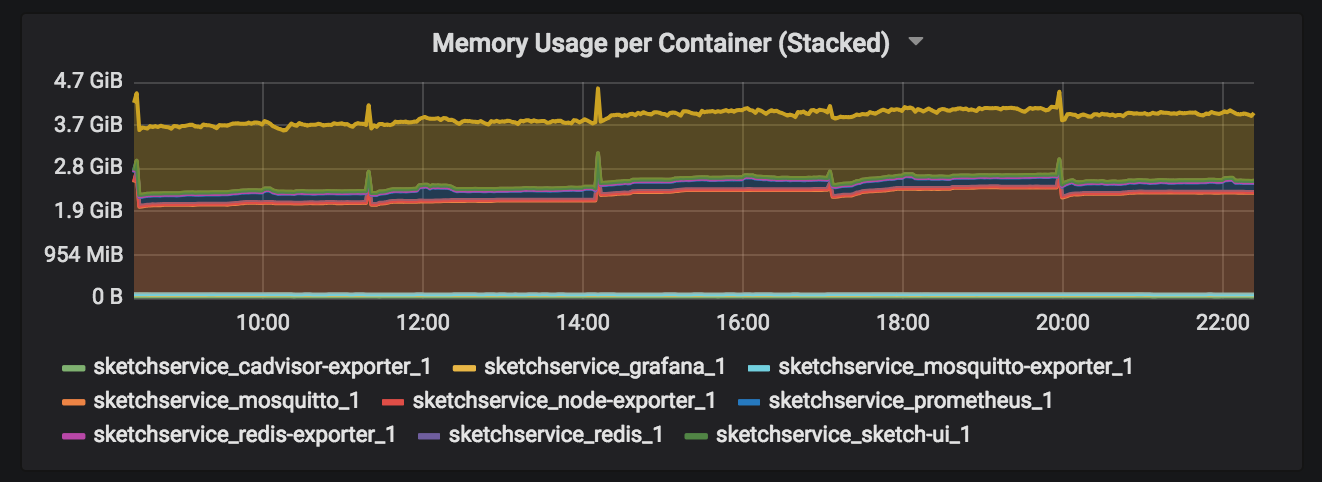
\includegraphics[width=1\textwidth]{./graph/memory_usage.png}
	\caption{Consumo de memoria de los contenedores.}
	\label{diag:memory_usage}
\end{figure}
\clearpage

\section{Instalación}
El sistema y sus dependencias se implementan usando \textit{docker-compose}\footnote{https://docs.docker.com/compose/}. Esto permite su distribución de manera sencilla y asegura independencia del sistema operativo y servidor donde es ejecutado. Las instrucciones para su instalación, configuración y prueba pueden encontrarse en \hyperref[https://github.com/leandropineda/sketch-service]{https://github.com/leandropineda/sketch-service}. Las instrucciones para instalar \textit{docker} y \textit{docker-compose} pueden encontrarse en su página oficial \hyperref[https://www.docker.com/]{https://www.docker.com/}

\

El código fuente del servicio está disponible en \hyperref[https://github.com/leandropineda/sketch-ws]{https://github.com/leandropineda/sketch-ws}. La imagen Docker, que se construye automáticamente con cada nuevo commit al repositorio Git, está disponible en \hyperref[https://hub.docker.com/r/lpineda/sketch-ws/]{https://hub.docker.com/r/lpineda/sketch-ws/}. Puede descargarse del registro público usando el comando \textit{docker pull lpineda/sketch-ws}.

\

De la misma manera, el código fuente de la interfaz web puede encontrarse en \hyperref[https://github.com/leandropineda/sketch-ui]{https://github.com/leandropineda/sketch-ui}, y la imagen docker correspondiente está disponible en \hyperref[https://hub.docker.com/r/lpineda/sketch-ui/]{https://hub.docker.com/r/lpineda/sketch-ui/}. El comando para descargar la imagen del repositorio público es \textit{docker pull lpineda/sketch-ui}.


\clearpage
\section{Conclusiones}
Para un flujo de eventos representados como cadenas de caracteres el sistema permite identificar en tiempo real aquellos eventos considerados como \textit{heavy keys}. Codificando los eventos de esta manera agregó complejidad a su desarrollo, pero a su vez el sistema es lo suficientemente flexible para pueda ser integrado en diferentes aplicaciones sin dificultad. En términos del problema tratado y la solución propuesta, podemos concluir que el valor que la misma entrega al usuario radica en al velocidad a la que genera resultados, dado que como el costo de almacenar información hoy en día es sumamente bajo y abundan las soluciones basadas en \textit{bigdata}.

Respecto a la instalación del sistema vemos que no ofrece dificultad alguna dado que esta diseñado como un microservicio. Los contenedores Docker funcionan en cualquier sistema operativo y pueden desplegarse tanto en infraestructura propia del usuario como en el \textit{cloud}.

Es posible modificar las propiedades de los parámetros de detección del sistema usando un archivo de configuración según los datos que se quieren procesar. Los umbrales de detección deben ser configurados acorde a la aplicación, pero podría implementarse un mecanismo de ajuste automático (ver Trabajos futuros).

Podemos observar que las mejoraras en \textit{performance} son más que satisfactorias. Si bien para el presente informe sólo se usaron datos sintéticos y de tráfico de red, el mismo método puede aplicarse en diferentes aplicaciones. Por otro lado, la integración de una \textit{message queue} en el sistema fue fundamental, no solo para incrementar las prestaciones del servicio, sino para permitir escalabilidad: ante grandes volúmenes de eventos enviados al servicio, la carga es soportada por la \textit{message queue}, lo cual evita agregar esta lógica al servicio desarrollado.

La interfaz web muestra, en una sola vista, toda la actividad detectada por el sistema y permite a usuario observar cual es el estado 
general de los eventos que está analizando, sin necesidad de interactuar con la interfaz.

Finalmente, es importante resaltar el papel de la telemetría en este tipo de soluciones y la cantidad de ingeniería que su despliegue involucra. Es un aspecto fundamental de cualquier sistema que pretende usarse de manera ininterrumpida y al que solo se tenga acceso de manera remota. Así, si bien gran parte de la infraestructura actual del sistema fue implementada solo para estos fines, y se agrega cierta complejidad al código para que la misma pueda ser desplegada adecuadamente, el valor que entrega a los usuarios es de gran importancia.

\clearpage

\section{Trabajos futuros}
Respecto a la implementación del sistema:
\begin{itemize}
	\item Esta implementación usa umbrales que son definidos antes de iniciar el procesamiento de los datos. Esto no supone una limitación dado que aquellos responsables de las infraestructuras a monitorear usualmente tienen una buena idea que implica una anomalía y son capaces de elegir umbrales suficientemente buenos como para lograr resultados adecuados. Sin embargo, es deseable desarrollar algún método por el cual estos parámetros se ajusten dinámicamente, de forma de hacer al sistema agnóstico de la aplicación donde se lo pretende usar.
	\item Los \textit{sketches} son estructuras basadas en proyecciones lineales, y por lo tanto se pueden realizar combinaciones lineales con los mismos. Esto permitiría soportar una arquitectura de detección distribuida, donde cada instancia del servicio procesa una parte de los eventos generados, para luego agregar los resultados de todas las instancias. De esta manera, puede agregarse redundancia y escalabilidad horizontal a la solución. La implementación de la base de datos clave-valor es un paso en esa dirección, dado que permite contar con un repositorio centralizado donde almacenar las asociaciones de cadenas de caracteres a números enteros.
	\item Además, al ser matrices de 2 dimensiones, los \textit{sketches} pueden pensarse como imágenes. Existen una miriada de métodos de procesamiento digital de imágenes para entender como éstas varían en el tiempo (podemos pensar una sucesión de épocas como un video, donde cada \textit{sketch} es un \textit{frame}). Resultaría interesante evaluar que conclusiones pueden obtenerse al intentar identificar anomalías bajo este enfoque.
\end{itemize}

Fuera de la aplicación en detección de ataques a redes de datos, este sistema podría adaptarse a \textit{e-commerce}: es posible instrumentar sitios web para determinar en tiempo real artículo es el mas buscado o más visto, donde cada evento sería el enlace que un usuario accede. Además, podría adaptarse a análisis de texto en tiempo real, para determinar que palabras son las más utilizadas en una red social, o cual es la palabra clave más utilizada en un motor de búsqueda dado.

\clearpage\mbox{}\clearpage
\section{Apéndices}

\subsection{Funciones de hash}
Una función hash $H$ es una función computable mediante un algoritmo tal que $H: M \rightarrow N$ y $x \rightarrow h(x)$. Tiene como entrada un conjunto de elementos, que suelen ser cadenas de caracteres, y los convierte en un rango de salida finito, que son normalmente cadenas de caracteres de longitud fija. Es decir, la función actúa como una proyección del conjunto $M$ sobre el conjunto $N$.

Decimos que existe una colisión cuando dos entradas distintas a una función de hash producen la misma salida. Es matemáticamente imposible que una función de hash carezca de colisiones, ya que el número potencial de posibles entradas es mayor que el número de salidas que puede producir un hash. Sin embargo, las colisiones se producen más frecuentemente en los malos algoritmos. En ciertas aplicaciones especializadas con un relativamente pequeño número de entradas que son conocidas de antemano es posible construir una función de hash perfecta, que se asegura que todas las entradas tengan una salida diferente. Pero en una función en la cual se puede introducir datos de longitud arbitraria y que devuelve un hash de tamaño fijo (como MD5), siempre habrá colisiones, debido a que un hash dado puede pertenecer a un infinito número de entradas.

Observar que $N$ puede ser un conjunto definido de enteros. En este caso podemos considerar que la longitud es fija si el conjunto es un rango de números de enteros ya que podemos considerar que la longitud fija es la del número con mayor número de cifras. Todos los números se pueden convertir al número especificado de cifras simplemente anteponiendo ceros.

Normalmente el conjunto $M$ tiene un número elevado de elementos y $N$ es un conjunto de cadenas con un número más o menos pequeño de símbolos. La idea básica de un valor hash es que sirva como una representación compacta de la cadena de entrada. Por esta razón se dice que estas funciones resumen datos del conjunto dominio.


\subsubsection{Familias de funciones de hash}
El objetivo de las funciones de hash es asociar elementos de un gran conjunto a otro más pequeño. En las estructuras de datos probabilísticas, usualmente es deseable que los códigos de hash se comporten de manera aleatoria, pues si se usan funciones de hash determinísticas un adversario podría escoger un conjunto de datos con las mismas pre-imágenes. Ademas, es posible que la elección de una función de hash determinística sea una mala elección para un conjunto de entrada dado (muchas colisiones): escoger aleatoriamente funciones de hash de una familia de funciones evita este problema dado que si bien puede escogerse una función con esta característica, lo más probable es que solo sea un caso asilado.
Existe una familia de funciones que asegura baja probabilidad de colisiones para un conjunto dado de elementos y comportamiento uniforme en la distribución de las pre-imágenes de los elementos\cite{WEGMAN1981265}.

Podríamos imaginarnos un algoritmo probabilístico de tiempo polinomial con dos mensajes codificados en el algoritmo que dan lugar a una colisión para una específica función resumen. El algoritmo simplemente devolvería los dos mensajes que causan la colisión. Crear tal algoritmo puede ser extremadamente difícil, pero una vez construido podría ser ejecutado en tiempo polinomial. Sin embargo, definiendo una familia de funciones de hash como una familia infinita de funciones hash impide que la búsqueda de este algoritmo tenga éxito para todas las funciones resumen de la familia, porque hay infinitas. Por tanto las familias resumen proporcionan un mecanismo interesante para el estudio y categorización de las funciones resumen respecto a su fortaleza frente a la búsqueda de colisiones por parte de un adversario. Este tipo de estudios es muy útil en el campo de la criptografía para los llamados códigos de detección de modificaciones.


\subsubsection{Familias de funciones de hash resistentes a colisiones}
De forma informal una familia de funciones es familia de funciones de hash resistente a colisiones, también llamadas CRHF por sus siglas en inglés (Collision Resistant Hash Function), si dada una función escogida aleatoriamente de la familia un adversario es incapaz de obtener una colisión para ella\cite{chunyuean}.

A continuación se describen familias de funciones de hash relevantes para este trabajo:
\subsubsection{Funciones de hash universales}
La definición de hash universal hace referencia a la propiedad para la cual dos elementos distintos no colisionan muy a menudo. Fue propuesta por Carter y Wegmar en 1979\cite{WEGMAN1981265}.


\paragraph{Definición} Sea $M = \{0, 1, \dots m-1 \}$ y $N = \{0, 1, \dots n-1 \}$ con $m \geq n$. Una familia $H$ de funciones de $M$ a $N$ is \textit{2-universal} si, para todo $x,y \in M$ tal que $x\neq y$, y para $h$ elegido uniformemente al azar de $H$, tenemos que: 

\begin{equation}
	\mathcal{P}[h(x) = h(y)] \leq \frac{1}{n}
\end{equation}
Esta condición debe cumplirse para \textit{todo par} de elementos diferentes, y la aleatoriedad es sobre la elección de la función de hash $h$ del conjunto $H$.

Una asociación completamente aleatoria de $M$ a $N$ tiene una probabilidad de colisión de exactamente $1/n$; por lo tanto, una función elegida al azar de una familia \textit{2-universal} de funciones de hash da una función aproximadamente aleatoria. La colección de todas las funciones de $M$ a $N$ es una familia \textit{2-universal}, pero tiene algunas desventajas: elegir una función de manera aleatoria de este conjunto requiere $\Omega(m \log n)$ bits aleatorios. Esto es además la cantidad de bits de memoria requeridos para representar la función elegida. Es deseable obtener familias de funciones \textit{2-universales} mas pequeñas que requieran menor cantidad de espacio y que sean fáciles de evaluar; en particular, queremos construir familias de funciones \textit{2-universales} que contengan solo un pequeño subconjunto de todas las funciones posibles. La razón por la cual esto es posible es por que una función elegida al azar $h \in H$ debe comportarse como aleatoria solo con respecto a pares de elementos. Si hacemos variar $x$ sobre $M$, los valores $h(x)$ se comportan casi como variables independientes de a pares, razón por la cual se llaman \textit{2-universales}. Por otro lado, para una función $f$ completamente aleatoria, los valores $f(x)$ tienen independencia completa. Las familias de funciones de hash 'fuertemente' \textit{2-universales} tienen una correspondencia exacta con variables aleatorias independientes de a pares.

\

A continuación introduciremos las herramientas necesarias para desarrollar un método de construcción de funciones de hash \textit{2-universales}. Sean $M$, $N$ y $H$. Para cualquier $x,y \in M$ y $h \in H$, definimos la siguiente función que indica la colisión entre los elemento $x$ e $y$ para la función $h$:

\begin{equation}
	\delta(x,y,h) = \left\{
								\begin{array}{ll}

									1 & \text{para} \ h(x) = h(y) \ \text{y} \ x \neq y \\
									0 & \text{de otra manera}
								\end{array}
							\right.
\end{equation}

Para todo $X, Y \subseteq M$, definimos las siguientes extensiones de la función indicador $\delta$:

\begin{equation}
	\begin{array}{lll}
		\delta(x,y,H) & = & \sum\limits_{h \in H} \delta(x,y,h) \\[0.5cm]
		\delta(x,Y,h) & = & \sum\limits_{y \in Y} \delta(x,y,h) \\[0.5cm]
		\delta(X,Y,h) & = & \sum\limits_{x \in X} \delta(x,Y,h) \\[0.5cm]
		\delta(x,Y,H) & = & \sum\limits_{y \in Y} \delta(x,y,H) \\[0.5cm]
		\delta(X,Y,H) & = & \sum\limits_{h \in H} \delta(X,Y,h) \\
	\end{array}
\end{equation}

Si $H$ es una familia \textit{2-universal} y para cualquier $x \neq y$, tenemos que $\delta(x,y,H) \leq |H|/n$.
El siguiente teorema muestra que la definición de \textit{2-universalidad} es esencialmente la mejor posible, dado que no se pueden obtener probabilidades de colisión menores para $m \gg n$ (al menos no significativas).

\begin{theorem}

	Para cualquier familia $H$ de funciones de $M$ a $N$, existe $x, y \in M$ tal que:
	\begin{equation}
		\delta(x,y,H) > \frac{|H|}{n} - \frac{|H|}{m}
	\end{equation}
\end{theorem}

\begin{proof}
	Sea $h$ una función tal que $h \in H$, y para cada $z \in N$ definimos el conjunto de elementos de $M$ con imagen $z$ como
	\begin{equation}
		A_z = \{  x \in M | h(x) = z \}
	\end{equation}
	
	Los conjuntos $A_z$, para $z \in N$, forman una partición de $M$. Es fácil verificar que:
	
	\begin{equation}
		\delta(A_w,A_z,h) = \left\{
									\begin{array}{cl}
										0 & w \neq z \\
										|A_z|(|A_z| - 1) & w=z
									\end{array}
								\right.
	\end{equation}
	
	Esto es así porque para que dos elementos cualesquiera colisionen, ambos deben pertenecer al mismo conjunto $A_z$, y el número de colisiones entre los elementos de $A_z$ es exactamente $|A_z|(|A_z| - 1)$. El número total de colisiones entre todos los pares posibles de elementos se minimiza cuando los conjuntos $A_z$ son todos del mismo tamaño. Tenemos que:
	
	\begin{equation}
		\begin{array}{ll} 
			\delta(M,M,h) & = \sum\limits_{z \in N} |A_z|(|A_z| - 1) \\[0.5cm]
									& \geq n (\frac{m}{n} (\frac{m}{n} - 1)) = m^2(\frac{1}{n}-\frac{1}{m})
		\end{array}
	\end{equation}
	
	El cálculo de $\delta(M,M,h)$ vale para una única función $h \in H$, y por lo tanto $\delta(M,M,H) = \sum_{h \in H} \delta(M,M,h) \geq |H|m^2(1/n-1/m)$. Por el principio del palomar, debe existir un par de elementos $x, y \in M$ tal que:
	
	\begin{equation}
		\begin{array}{ll}
			\delta(x,y,H) & \geq \frac{\delta(M,M,H)}{m^2} \\[0.5cm]
								  & = \frac{|H|\delta(M,M,h)}{m^2} \\[0.5cm]
								  & \geq \frac{|H|m^2(1/n-1/m)}{m^2}\\[0.5cm]
								  & = |H|(\frac{1}{n}-\frac{1}{m})_{\qed}
		\end{array}
	\end{equation}

\end{proof}

\subsubsection{Construcción de una familia de funciones de hash universal}
La construcción de familias de hash \textit{2-universales} es algebraica. Dados $m$ y $n$, sea $p$ un número primo tal que $p \geq m$. Sea $\mathbf{Z}_p = \{ 0, 1, \dots, p-1\}$ y $g: \mathbf{Z}_p \rightarrow N$ la función dada por $g(x) = x \mod n$. Para todo $a,b \in \mathbf{Z}_p$ definimos la función $f_{a,b}: \mathbf{Z}_p \rightarrow \mathbf{Z}_p$ y la función de hash $h_{a,b}: \mathbf{Z}_p \rightarrow N$ como sigue:

\begin{equation}
	\begin{array}{ll}
		f_{a,b} = & ax + b \mod p \\
		h_{a,b} = & g(f_{a,b}(x))
	\end{array}
\end{equation}

Definimos la familia de funciones de hash $H = \{ h_{a,b} | a,b \in \mathbf{Z}_p \ \text{con} \ a \neq 0 \}$ y decimos que es \textit{2-universal}. Aunque $H$ usa $\mathbf{Z}_p$ como su dominio, la definición anterior aplica para cualquier subconjunto de $\mathbf{Z}_p$, en particular el dominio $M$.

\begin{lemma}\label{lemma:pair_colisions}

	Para todo $x,y \in \mathbf{Z}_p$ tal que $x \neq y$:
	\begin{equation}
		\delta(x,y,H) = \delta(\mathbf{Z}_p,\mathbf{Z}_p,g)
	\end{equation}
\end{lemma}
\begin{proof}
	Mostraremos que el número de funciones en $H$ que causan colisión entre $x$ e $y$ está determinado por el tamaño de las clases residuo de $\mathbf{Z}_p \pmod{n}$. Las clases residuo de una función $f(x) \pmod{n}$ son todos los valores posibles del residuo de $f(x) \pmod{n}$. Por ejemplo, las clases residuo de $x^2 \pmod{6}$ son $\{ 0, 1, 3, 4 \}$ dado que todos los residuos posibles son:
	\begin{equation}
		\begin{array}{lll}
			0^2 & \equiv & 0 \pmod{6}\\		
			1^2 & \equiv & 1 \pmod{6}\\	
			2^2 & \equiv & 4 \pmod{6}\\	
			3^2 & \equiv & 3 \pmod{6}\\	
			4^2 & \equiv & 4 \pmod{6}\\	
			5^2 & \equiv & 1 \pmod{6}
		\end{array}
	\end{equation}
	
	Supongamos que $x$ e $y$ colisionan bajo una función específica $h_{a,b}$. Sea $f_{a,b}(x) = r$ y $f_{a,b}(y) = s$, y obsérvese que $r\neq s$ dado que $a \neq 0$ y $x \neq y$. Una colisión solo puede producirse si y solo si $g(r) = g(s)$, o de manera equivalente, si $r \equiv s \pmod{n}$. Ahora, con $x$ e $y$ fijos, para cada elección de $r$ y $s$ tal que $r \neq s$, los valores de $a$ y $b$ quedan determinados de manera única como la solución del siguiente sistema lineal de ecuaciones en $\mathbf{Z}_p$:
	
	\begin{equation}
		\begin{array}{lll}
			ax+b & \equiv & r \pmod{p} \\
			ay+b & \equiv & s \pmod{p}
		\end{array}
	\end{equation}
	
	Por lo tanto, el número de funciones de hash $h_{a,b}$ que causan que $x$ e $y$ colisionen es exactamente el número de elecciones de $r$ y $s$ ($r \neq s$) tales que $r \equiv s \pmod{n}$. Y esto está dado por $\delta(\mathbf{Z}_p,\mathbf{Z}_p,g)_{\qed}$.
\end{proof}
\


\begin{theorem}
	La familia de funciones de hash $H={h_{a,b} | a, b \in \mathbf{Z}_p \ \text{con} \ a \neq 0}$ es \textit{2-universal}.
\end{theorem}
\begin{proof}
	Para cada $z \in N$, sea $A_z = \{ x \in \mathbf{Z}_p | g(x) = z \}$. Es claro que $|A_z| \leq \lceil p/n \rceil$. En otras palabras, para cada $r \in \mathbf{Z}_p$ existen al menos $\lceil p/n \rceil$ elecciones diferentes de $s \in \mathbf{Z}_p$ tal que $g(r) = g(s)$. Dado que hay $p$ elecciones diferentes de $r \in \mathbf{Z}_p$ para empezar,
	\begin{equation}
		\delta(\mathbf{Z}_p,\mathbf{Z}_p,g) \leq p \left( \lceil p/n \rceil - 1 \right) \leq \frac{p(p-1)}{n}
	\end{equation}
	
	El lema \ref{lemma:pair_colisions} implica que para cualesquiera $x$ e $y$ en $\mathbf{Z}_p$, $\delta(x,y,H) \leq p(p-1)/n$. Dado que el tamaño de $|H|$ es exactamente $p(p-1)$, tenemos que $\delta(x,y,H) \leq |H|/n$. \qed
\end{proof}

Un resultado conocido en la teoría de números es el postulado de Bertrand el cual dice que para cualquier entero $m$, existe un número primo entre $m$ y $2m$. Entonces podemos elegir $p = O(m)$, y el número de bits aleatorios necesarios para elegir una función de hash de $H$ no es mayor a $2 \log p = O(\log m)$. Elegir, almacenar y evaluar funciones de hash en $H$ es simple y eficiente. Solo es necesario elegir $a$ y $b$ de manera independiente y uniformemente al azar de $\mathbf{Z}_p$. Estos valores pueden ser almacenados en un mínimo de memoria y evaluar $h_{a,b}$ es una tarea trivial.

\

\subsection{Cabeceras de protocolos}

\subsubsection{Cabecera IP}
El protocolo de internet (en inglés Internet protocol o IP) es un protocolo de comunicación de datos digitales clasificado funcionalmente en la capa de red según el modelo internacional OSI.

Su función principal es el uso bidireccional en origen o destino de comunicación para transmitir datos mediante un protocolo no orientado a conexión que transfiere paquetes conmutados a través de distintas redes físicas previamente enlazadas según la norma OSI de enlace de datos.

\begin{figure*}[h]
	\centering
	\begin{bytefield}{32}
		\bitheader{0,3,4,7,8,15,16,18,19,23,24,31} \\
		\bitbox{4}{Version} &
		\bitbox{4}{IHL} &
		\bitbox{8}{\small Type of Service} &
		\bitbox{16}{Total Length} \\
		\bitbox{16}{Identification} &
		\bitbox{3}{Flags} &
		\bitbox{13}{Fragment Offset} \\
		\bitbox{8}{Time to Live} &
		\bitbox{8}{Protocol} &
		\bitbox{16}{Header Checksum} \\
		\bitbox{32}{Source Address} \\
		\bitbox{32}{Destination Address} \\
		\bitbox{24}{Options} &
		\bitbox{8}{Padding} \\
	\end{bytefield}
	\caption{Cabecera IP}
	\vspace{1cm}
\end{figure*}

\subsubsection{Cabecera TCP}

Protocolo de control de transmisión (en inglés Transmission Control Protocol o TCP), es uno de los protocolos fundamentales en Internet.

Muchos programas dentro de una red de datos compuesta por redes de computadoras, pueden usar TCP para crear “conexiones” entre sí a través de las cuales puede enviarse un flujo de datos. El protocolo garantiza que los datos serán entregados en su destino sin errores y en el mismo orden en que se transmitieron. También proporciona un mecanismo para distinguir distintas aplicaciones dentro de una misma máquina, a través del concepto de puerto.

TCP da soporte a muchas de las aplicaciones más populares de Internet (navegadores, intercambio de ficheros, clientes FTP, etc.) y protocolos de aplicación HTTP, SMTP, SSH y FTP.

\begin{figure*}[h]
	\centering
	\begin{bytefield}{32}
		\bitheader{0,15,31} \\
		\bitbox{16}{Source Port} &
		\bitbox{16}{Destination Port} \\
		\bitbox{16}{Sequence Number} &
		\bitbox{16}{Acknowlegment Number} \\
	\end{bytefield}
	\caption{Cabecera UDP}
	\vspace{1cm}
\end{figure*}

\subsubsection{Cabecera UDP}
El protocolo de datagramas de usuario (en inglés: User Datagram Protocol o UDP) es un protocolo del nivel de transporte basado en el intercambio de datagramas (Encapsulado de capa 4 o de Transporte del Modelo OSI). Permite el envío de datagramas a través de la red sin que se haya establecido previamente una conexión, ya que el propio datagrama incorpora suficiente información de direccionamiento en su cabecera. Tampoco tiene confirmación ni control de flujo, por lo que los paquetes pueden adelantarse unos a otros; y tampoco se sabe si ha llegado correctamente, ya que no hay confirmación de entrega o recepción. Su uso principal es para protocolos como DHCP, BOOTP, DNS y demás protocolos en los que el intercambio de paquetes de la conexión/desconexión son mayores, o no son rentables con respecto a la información transmitida, así como para la transmisión de audio y vídeo en real, donde no es posible realizar retransmisiones por los estrictos requisitos de retardo que se tiene en estos casos.

\begin{figure*}[h]
	\centering
	\begin{bytefield}{32}
		\bitheader{0,3,4,6,7,15,16,31} \\
		\bitbox{16}{Source Port} &
		\bitbox{16}{Destination Port} \\
		\bitbox{32}{Sequence Number} \\
		\bitbox{32}{Acknowlegment Number} \\
		\bitbox{4}{Offset} &
		\bitbox{3}{} &
		\bitbox{9}{Flags} &
		\bitbox{16}{Window Size} \\
		\bitbox{16}{Checksum} &
		\bitbox{16}{Urgent Pointer} \\
	\end{bytefield}
	\caption{Cabecera TCP}
\end{figure*}
%
\clearpage

\section{Anexos}

\begin{figure}[h!]
	\centering
	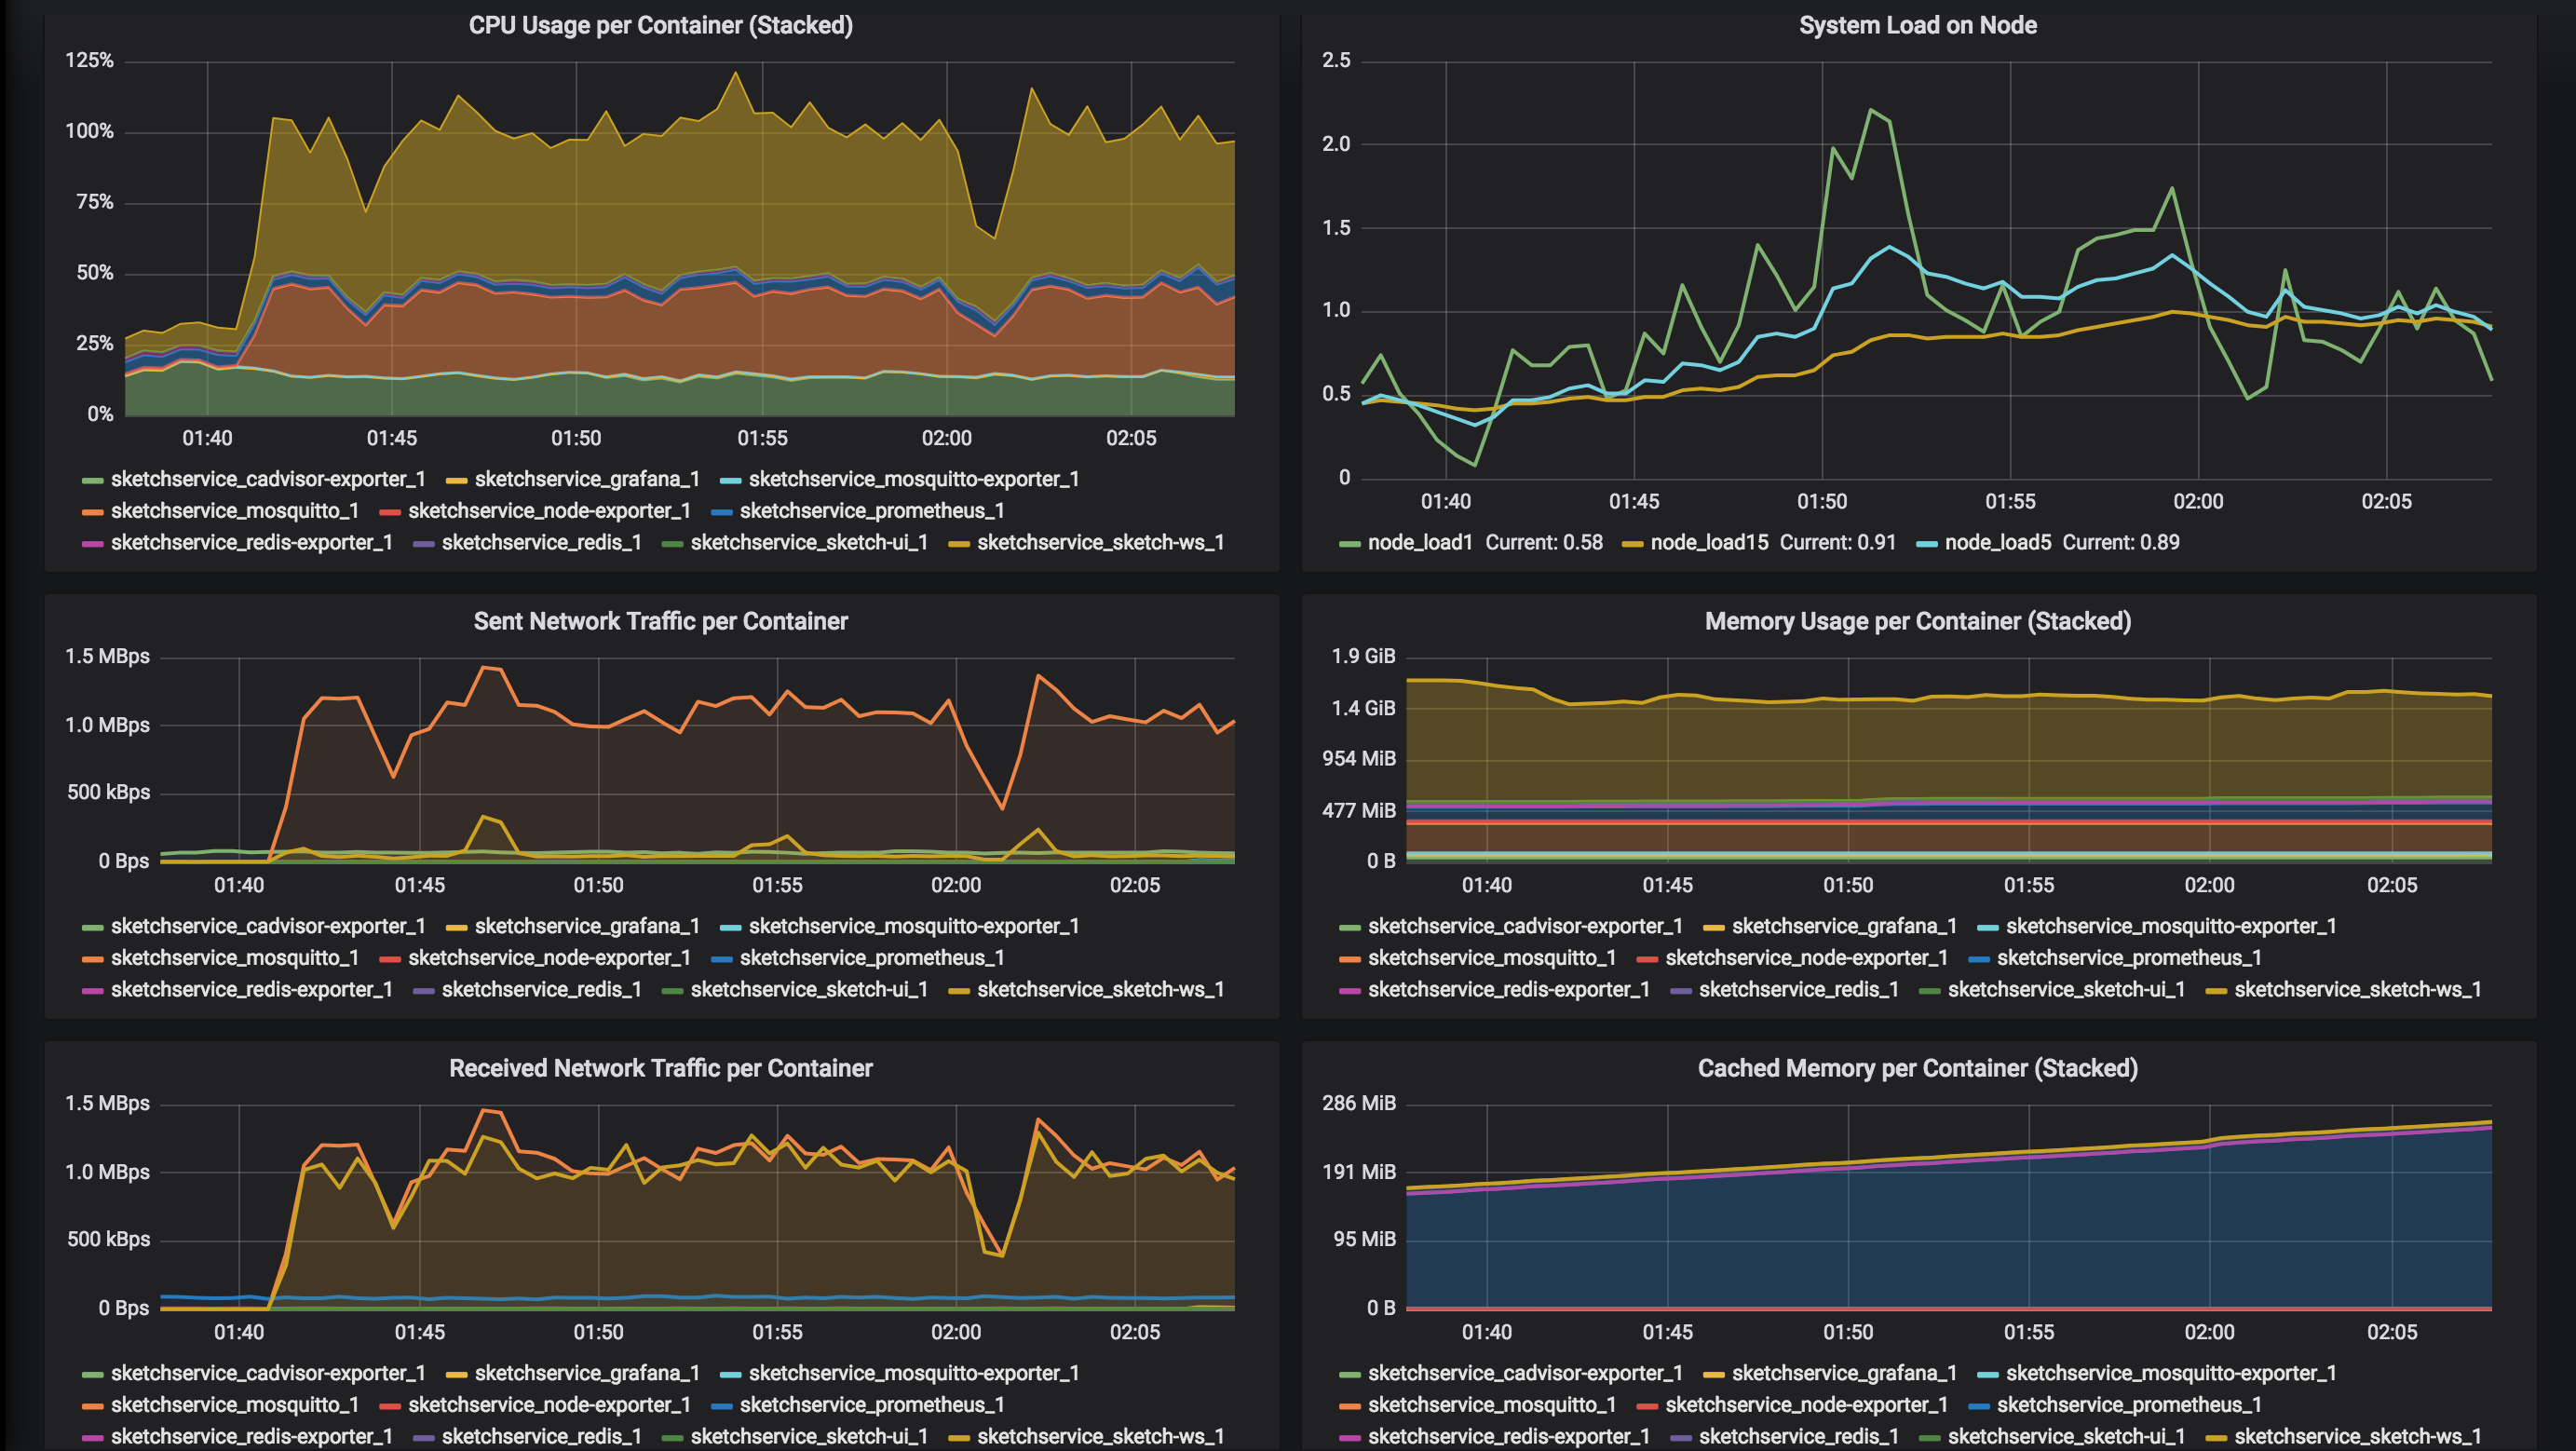
\includegraphics[width=1.5\textwidth,angle=90]{./graph/system_dashboard.png}
	\caption{Dashboard del sistema.}
	\label{diag:system_dashbard}
\end{figure}

\begin{figure}[h]
	\centering
	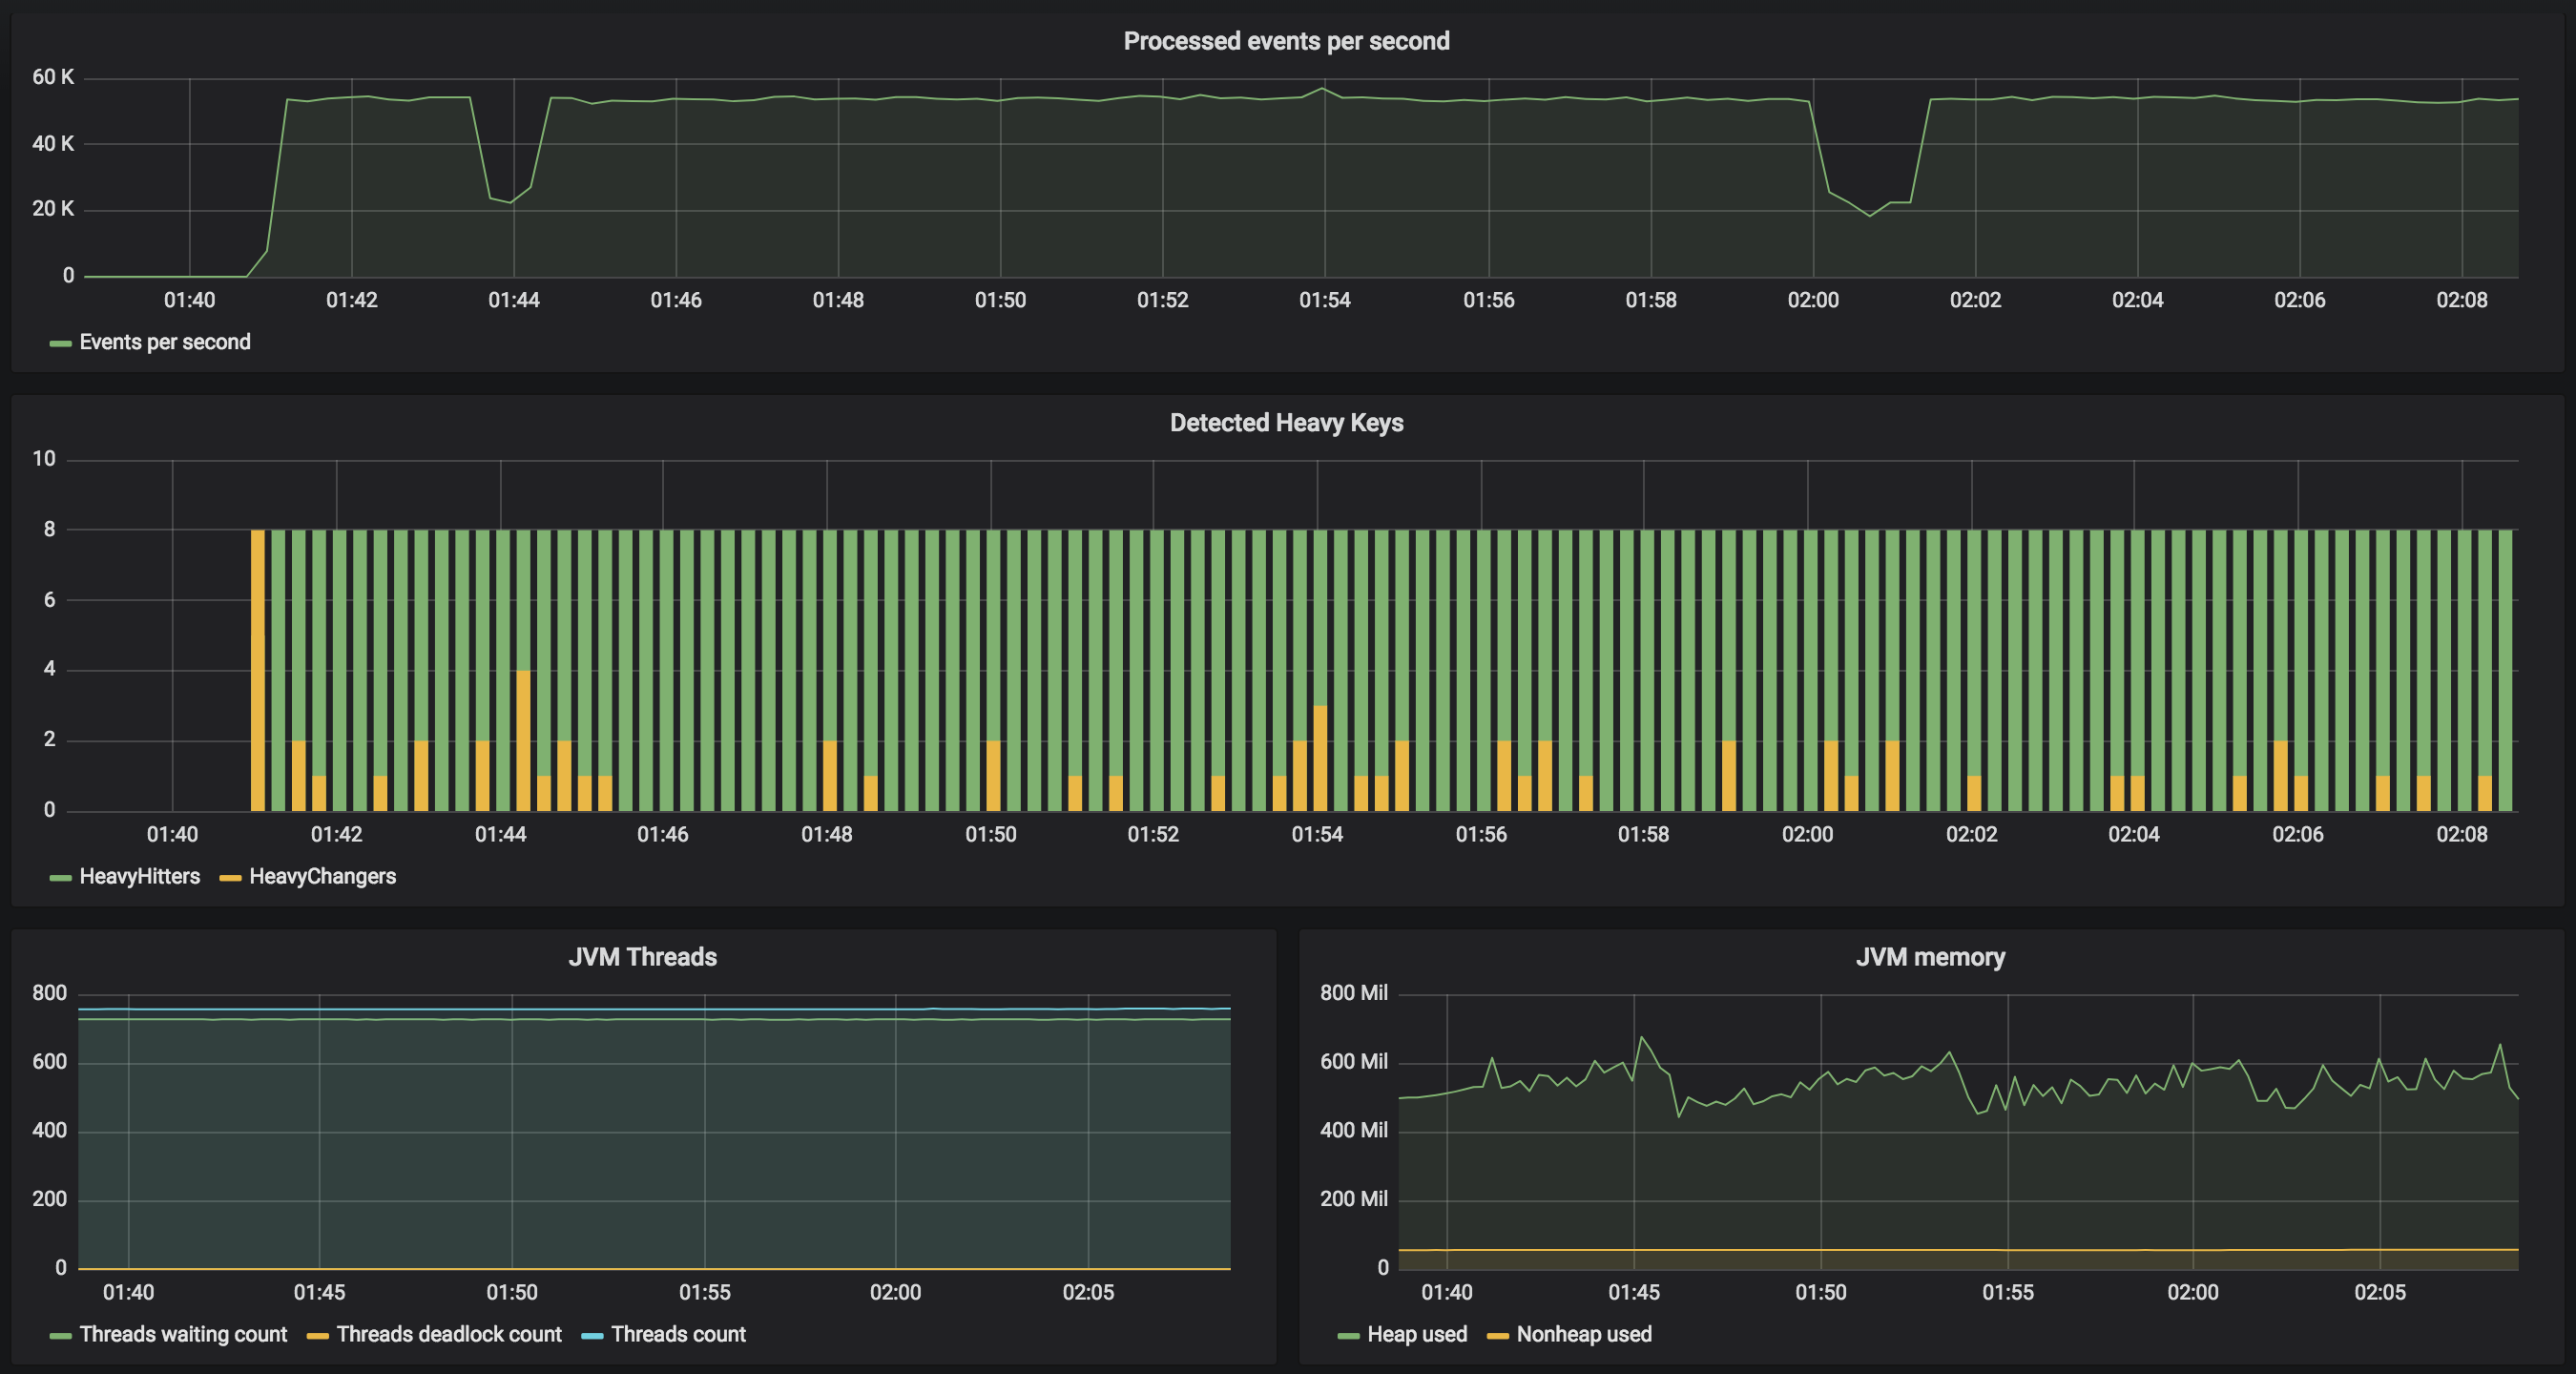
\includegraphics[width=1.5\textwidth,angle=90]{./graph/service_dashboard.png}
	\caption{Dashboard del servicio.}
	\label{diag:service_dashboard}
\end{figure}

\begin{figure}[h]
	\centering
	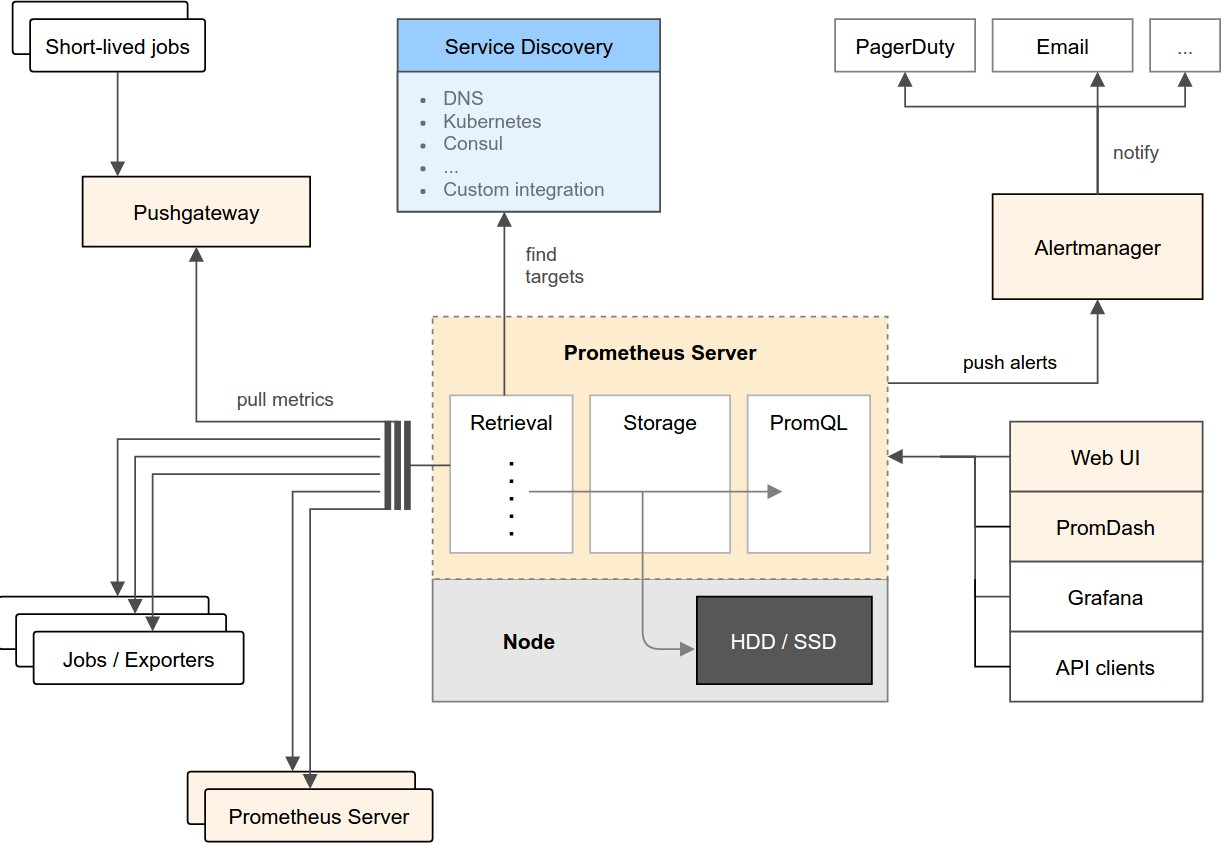
\includegraphics[width=1.2\textwidth,angle=90]{./graph/prometheus.jpeg}
	\caption{Arquitectura de Prometheus.}
	\label{diag:prometheus}
\end{figure}

\clearpage

\listoffigures

\clearpage

\nocite{*}
\printbibliography


\end{document}

